\chapter{Results}
\label{chapter: Results}

% REVIEW: chapter introduction still a placeholder.
Write Introduction paragraph 

\section{Angled Glass Experiment Results}
\label{section: Angled Glass Experiment Results}
The Angled Glass Experiment aimed to validate the methodology and compare the different defocus configurations treated in Chapter \ref{chapter: methodology}. This section presents the data gathered, describes how it was treated, discusses the uncertainty of the results, and concludes whether these objectives have been achieved. The tables that follow give an overview of the results.

Table \ref{tab: angled glass displacement results} compares the displacements measured through SBOS with the predicted shift induced by the angled glass. $\Delta_x$ is the mean of the cross-correlation vector field in pixels, $\Delta x_{SBOS}$ is the latter transferred to mm in the focal plane and $\Delta x_{glass}$ is the glass-induced ray shift, calculated through Equation \ref{equation: Displacement of angled glass}. Since the glass piece produces a uniform displacement field, the standard deviation of the cross-correlation field $\sigma_\Delta$ quantifies the precision of the SBOS measurement, while the relative error quantifies the accuracy of the method. The last column displays the total combined uncertainty of measurement of $\Delta x$, which will be treated in more detail later this section.

The table allows the comparison of the measurement error with its inherent uncertainty. In general terms, the error obtained is below the combined uncertainty, with the exception of points 1, 17 and 18. Only point 1, however, differs significantly from the uncertainty, with a difference of 4.76 percentage points, while 17 and 18 deviate by less than 0.5 percentage points. Regarding point 1, an error of $1.26^{\circ}$ in the glass angle measurement would be needed to cause its deviation of 7.87\%, which exceeds the reading uncertainty of the protractor. The cause for such error could be a misread angle or an unnoticed movement that changed the angle when setting it in the rail.

% REVIEW: "every point except 1 stays ... below its measurement uncertainties" contradicts the previous paragraph, where points 17 and 18 exceed their uncertainty.
The slider experimental error is also worth a remark due to the distinct behavior of its deviation. As it can be seen in Table \ref{tab: angled glass displacement results}, all the deviations of the slider experiments are positive and have a similar magnitude, which leads to the interpretation of an induced bias in the measurement. It is not clear what caused this bias, although it could have been introduced by an error in the magnification added to one in the glass angle, as both were fixed throughout the measurements. Nevertheless, the deviation of every point except 1 stays well within 5\%, below its measurement uncertainties, and the scatter signaled by $\sigma_\Delta$ is well within 2px. Consequently, these metrics indicate that the technique has been well implemented and is capable of producing accurate and precise results.

%Alternative for the above paragraph
%Every point except point 1 falls within its own standard uncertainty, and points 17 and 18 are the only ones that require the interval defined by $k = 2$. The agreement is therefore better than the raw percentages suggest, since the points with the largest deviations are also the ones with the largest scatter. Point 1 is the exception at 7.87\%, which is 2.5 times its combined standard uncertainty of 3.11\%. The glass angle alone does not explain it, because an error of $1.26^{\circ}$ would be required and that value exceeds the reading uncertainty of the protractor by more than a factor of four. The most likely explanation is a combination of a misread angle and a plate that was not seated flat against its mount. not seated flat against it mount? What?


\begin{table}[h]
    \centering
    \caption{Displacements measured in the angled glass campaigns. $\Delta_x$ is the mean displacement returned by the cross-correlation, $\sigma_\Delta$ its standard deviation over the vector field, $\Delta x_{SBOS}$ is that displacement referred to the focal plane, $\Delta x_{glass}$ the value calculated by Equation \ref{equation: Displacement of angled glass} for a plate of thickness $T = 2$ mm and refractive index $n = 1.52$ at the measured angle $\theta$. The $\Delta x_{SBOS}$ dev. column is the relative deviation of the two. Points 1 to 9 follow the fixed field of view configurations of Table \ref{tab: angled glass test matrix}; points 10 to 20 follow the linear slider configurations of the same table. The column $u_{tot}$ gives the combined standard uncertainty of the comparison between $\Delta x_{SBOS}$ and $\Delta x_{glass}$ calculated from the budgets of Tables \ref{tab: angled glass uncertainty} and \ref{tab: measurement uncertainty}.}
    \label{tab: angled glass displacement results}
    \begin{tabular}{lrrrrrrr}
        \toprule
        Point & $\theta$ & $\Delta_x$ & $\sigma_\Delta$ & $\Delta x_{SBOS}$ & $\Delta x_{glass}$ & $\Delta x_{SBOS}$ dev. & $u_{tot}$ \\
              & [$^{\circ}$] & [px] & [px] & [mm] & [mm] & [\%] & [\%] \\
        \midrule
         1 & 17 & 29.818 & 0.6001 & 0.1933 & 0.2099 & $-7.87$ &  3.11 \\
         2 & 17 & 22.613 & 1.3660 & 0.2136 & 0.2099 & $+1.77$ &  6.49 \\
         3 & 17 & 34.355 & 0.8521 & 0.2137 & 0.2099 & $+1.84$ &  3.43 \\
         4 & 17 & 21.368 & 0.5763 & 0.2071 & 0.2099 & $-1.30$ &  3.59 \\
         5 & 17 & 33.414 & 0.7710 & 0.2082 & 0.2099 & $-0.78$ &  3.31 \\
         6 & 17 & 23.067 & 1.0230 & 0.2088 & 0.2099 & $-0.51$ &  5.03 \\
         7 & 20 & 41.386 & 1.8830 & 0.2552 & 0.2500 & $+2.05$ &  5.05 \\
         8 & 20 & 22.306 & 0.6617 & 0.2537 & 0.2500 & $+1.46$ &  3.68 \\
         9 & 20 & 25.238 & 0.7720 & 0.2565 & 0.2500 & $+2.59$ &  3.76 \\
        \midrule
        10 & 20 & 29.373 & 0.7733 & 0.2561 & 0.2500 & $+2.42$ &  3.42 \\
        11 & 20 & 29.432 & 0.8055 & 0.2566 & 0.2500 & $+2.63$ &  3.50 \\
        12 & 20 & 29.595 & 0.7575 & 0.2580 & 0.2500 & $+3.20$ &  3.36 \\
        13 & 20 & 29.613 & 0.7711 & 0.2582 & 0.2500 & $+3.26$ &  3.40 \\
        14 & 20 & 29.580 & 0.7661 & 0.2579 & 0.2500 & $+3.15$ &  3.39 \\
        15 & 20 & 29.662 & 0.8175 & 0.2586 & 0.2500 & $+3.43$ &  3.51 \\
        16 & 20 & 29.559 & 0.7815 & 0.2577 & 0.2500 & $+3.07$ &  3.43 \\
        17 & 20 & 29.653 & 0.7694 & 0.2585 & 0.2500 & $+3.40$ &  3.39 \\
        18 & 20 & 29.746 & 0.7815 & 0.2593 & 0.2500 & $+3.73$ &  3.41 \\
        19 & 20 & 29.653 & 0.8264 & 0.2585 & 0.2500 & $+3.40$ &  3.54 \\
        20 & 20 & 29.617 & 0.8570 & 0.2582 & 0.2500 & $+3.28$ &  3.62 \\
        \bottomrule
    \end{tabular}
\end{table}

Through Table \ref{tab: df and Mag angled glass results}, the design strategy of Chapter \ref{chapter: methodology} can be assessed. It presents a comparison of the optical distances and magnifications prescribed by the surface maps with the ones obtained through the focal plane calibration. In addition, the resulting $L_{FoV_{obj}}$ was compared with the enforced 17 mm field of view of the object. The table was restricted to the 9 points where the methodology of Chapter \ref{chapter: methodology} was used to size the optical setup. The relative magnification errors are all below 5\% with the exception of point 7. The latter was obtained using the minimum distance at which the calibration plate could be brought into focus when using an $f = 105$ mm lens. That distance was bigger than the one prescribed by the surface map, resulting in a large $d_f$, $M_{ag}$ and $L_{FoV_{obj}}$ error. The propagation of that error is also evident in the sensitivity shown in Table \ref{tab: sensitivity comparison}. Point 9 also deviates from the enforced field of view by more than 5\%, in this case by $-8.64$\%. It was acquired at $l = 150$ mm, the longest defocus distance of the campaign. Points 7 and 9 are therefore the two geometric extremes of the design space, the shortest focal length and the largest defocus, and they are also the only two points whose field of view falls outside 5\%. All remaining deviations are within that band, which signals the correct implementation of the method. The contribution of the optical magnification to the uncertainty was obtained through the maximum fit residual of the DaVis calibration and can be seen in Table \ref{tab: measurement uncertainty}.

\begin{table}[h]
    \centering
    \caption{Optical design values against measured values of the experimental campaign. $d_{f,th}$ and $M_{ag_{th}}$ are, respectively, the focal distance and optical magnification prescribed by the design methodology of Chapter \ref{chapter: methodology} and listed in Table \ref{tab: angled glass test matrix}. $M_{ag_{exp}}$ was measured with a calibration plate at the in-focus plane and $d_{f,exp}$ was calculated through $d_f = f(M_{ag_{exp}}+1)/M_{ag_{exp}}$. The $d_f$ and $M_{ag}$ deviation columns are the relative difference with respect to the design value. $L_{FoV_{obj}}$ is the field of view achieved at the refractive object, obtained from Equation \ref{equation: LFoVobj BOS} with the experimental magnification. Its deviation was taken with respect to the 17 mm $L_{FoV_{obj}}$ enforced during the design.}
    \label{tab: df and Mag angled glass results}
    \begin{tabular}{lrrrrrrrr}
        \toprule
        Point & $d_{f,th}$ & $d_{f,exp}$ & $d_f$ dev. & $M_{ag_{th}}$ & $M_{ag_{exp}}$ & $M_{ag}$ dev. & $L_{FoV_{obj}}$ & $L_{FoV_{obj}}$ dev. \\
              & [mm] & [mm] & [\%] & [--] & [--] & [\%] & [mm] & [\%] \\
        \midrule
        1 & 409.0 & 399.5 & $-2.32$ & 0.9561 & 1.0025 &  $+4.85$ & 16.81 & $-1.12$ \\
        2 & 505.0 & 490.6 & $-2.85$ & 0.6557 & 0.6882 &  $+4.96$ & 17.07 & $+0.43$ \\
        3 & 391.0 & 391.4 & $+0.11$ & 1.0498 & 1.0449 &  $-0.47$ & 16.87 & $-0.76$ \\
        4 & 511.0 & 498.2 & $-2.50$ & 0.6433 & 0.6706 &  $+4.24$ & 16.73 & $-1.56$ \\
        5 & 393.0 & 391.7 & $-0.32$ & 1.0369 & 1.0431 &  $+0.59$ & 16.21 & $-4.65$ \\
        6 & 490.0 & 478.5 & $-2.35$ & 0.6897 & 0.7181 &  $+4.12$ & 16.28 & $-4.22$ \\
        7 & 189.0 & 204.6 & $+8.25$ & 1.2500 & 1.0543 & $-15.66$ & 18.52 & $+8.97$ \\
        8 & 285.0 & 288.7 & $+1.30$ & 0.5831 & 0.5715 &  $-1.98$ & 17.76 & $+4.46$ \\
        9 & 527.0 & 512.7 & $-2.71$ & 0.6109 & 0.6395 &  $+4.69$ & 15.53 & $-8.64$ \\
        \bottomrule
    \end{tabular}
\end{table}

The data collected during the experimental campaign allows the assessment of sensitivity through two experimental routes. Table \ref{tab: sensitivity comparison} compares the theoretical sensitivity given by the surface map of Chapter \ref{chapter: methodology} to the sensitivity obtained through the geometry $S_{geom} = l \cdot M_{ag_{exp}}$ and the sensitivity obtained with the displacement data $S_\Delta = \Delta_x \cdot l_{px}/\varepsilon_{glass}$. With the exception of point 7, which has already been discussed, all data is within 8\% of agreement. It is worth noting that the $S_{geom}$ error is the same as the magnification error, while $S_\Delta$ stacks both the displacement measurement error and the geometric setup error. The total combined uncertainty of $S_\Delta$ has also been calculated and is displayed in the last column, most points are below $u_{tot}$ in magnitude or within 1\% to it with the exception of point 7 and 9. It is worth noting that most points whose error exceeds the total uncertainty belong to the slider experiment, which could have experienced a bias, as previously mentioned. Nevertheless, the data shows that the optical configuration parameters defined by the methodology of Chapter \ref{chapter: methodology} produce a setup with the predicted sensitivity within an acceptable error range. Therefore, it validates the methodology as it demonstrates that the physical setup reproduces the predicted performance.

\begin{table}[h]
    \centering
    \caption{Sensitivity obtained by two routes compared to theoretical sensitivity. $S_{th} = l M_{ag_{th}}$ is the design sensitivity of Table \ref{tab: angled glass test matrix}. $S_{geom} = l M_{ag_{exp}}$ is the sensitivity measured with the calibration plate, carrying the same deviation of Table \ref{tab: df and Mag angled glass results}. $S_{\Delta} = \Delta_x \cdot l_{px} / \varepsilon_{glass}$ follows from the displacements measured. The $S_{geom}$ dev. and $S_{\Delta}$ dev. columns give the deviation of $S_{geom}$ and $S_{\Delta}$ to $S_{th}$. The column $u_{tot}$ displays the combined standard uncertainty on $S_{\Delta}$ for each point, obtained from the budgets of Tables \ref{tab: angled glass uncertainty} and \ref{tab: measurement uncertainty}.}
    \label{tab: sensitivity comparison}
    \begin{tabular}{lrrrrrr}
        \toprule
        Point & $S_{th}$ & $S_{geom}$ & $S_{\Delta}$ & $S_{geom}$ dev. & $S_{\Delta}$ dev. & $u_{tot}$ \\
              & [mm] & [mm] & [mm] & [\%] & [\%] & [\%] \\
        \midrule
         1 &  76.5 &  80.2 &  73.9 &  $+4.84$ &  $-3.42$ &  3.19 \\
         2 &  52.5 &  55.1 &  56.0 &  $+4.87$ &  $+6.73$ &  6.53 \\
         3 & 105.0 & 104.5 & 106.4 &  $-0.49$ &  $+1.34$ &  3.48 \\
         4 &  64.3 &  67.1 &  66.2 &  $+4.29$ &  $+2.93$ &  3.64 \\
         5 &  83.0 &  83.4 &  82.8 &  $+0.54$ &  $-0.24$ &  3.39 \\
         6 &  55.2 &  57.4 &  57.2 &  $+4.08$ &  $+3.55$ &  5.08 \\
         7 & 100.0 &  84.3 &  86.1 & $-15.66$ & $-13.93$ &  5.10 \\
         8 &  46.6 &  45.7 &  46.4 &  $-1.88$ &  $-0.45$ &  3.75 \\
         9 &  91.6 &  95.9 &  98.4 &  $+4.73$ &  $+7.44$ &  3.78 \\
        \midrule
        10 &   0.0 &   0.0 &   0.0 &  --   &  -- &    -- \\
        11 &   7.4 &   7.5 &   7.7 &  $+0.75$ &  $+3.40$ &  6.75 \\
        12 &  14.8 &  14.9 &  15.4 &  $+0.75$ &  $+3.97$ &  4.43 \\
        13 &  22.2 &  22.4 &  23.1 &  $+0.75$ &  $+4.04$ &  3.90 \\
        14 &  29.6 &  29.8 &  30.8 &  $+0.75$ &  $+3.92$ &  3.68 \\
        15 &  37.0 &  37.3 &  38.6 &  $+0.75$ &  $+4.21$ &  3.70 \\
        16 &   7.4 &   7.5 &   7.7 &  $+0.75$ &  $+3.85$ &  6.71 \\
        17 &  14.8 &  14.9 &  15.4 &  $+0.75$ &  $+4.18$ &  4.45 \\
        18 &  22.2 &  22.4 &  23.2 &  $+0.75$ &  $+4.50$ &  3.92 \\
        19 &  29.6 &  29.8 &  30.8 &  $+0.75$ &  $+4.18$ &  3.82 \\
        20 &  37.0 &  37.3 &  38.5 &  $+0.75$ &  $+4.05$ &  3.80 \\
        \bottomrule
    \end{tabular}
\end{table}

\par Tables \ref{tab: angled glass displacement results} and \ref{tab: sensitivity comparison} both show total uncertainties that were obtained to better assess the measurement error. These values were computed through uncertainty budgets following the Guide to the Expression of Uncertainty in Measurement \cite{JCGM2008}. The campaign compared a displacement obtained by Equation \ref{equation: Displacement of angled glass} against the displacement measured by cross-correlation. Therefore, two budgets were constructed, one for the glass displacement and another for the CC measurement. Afterwards, the collected uncertainties were combined to obtain the sensitivity uncertainty. A description of each budget and the formulas used to assess the total contribution follows.

The glass displacement's uncertainty budget is summarized in Table \ref{tab: angled glass uncertainty}. It focuses on the three inputs of the angled glass displacement estimate, namely the plate thickness $T$, the plate angle $\theta$ and the refractive index $n$. Thickness was measured with a caliper and the angle was set with a protractor, while the refractive index was obtained from the literature for common glass. Each input was treated as a rectangular probability distribution of half-width $a$ with a standard uncertainty of $u = a/\sqrt{3}$. The sensitivity coefficients and contributions of each input variable regarding the two glass angles were also estimated based on Equation \ref{equation: Displacement of angled glass}. These coefficients measure how much a change in each variable affects the final displacement. They are also used to calculate the contribution of each variable to the combined uncertainty as it is equal to the sensitivity coefficient times uncertainty \cite{JCGM2008}. These quantities are presented in Table \ref{tab: angled glass uncertainty}, where the half-width and the standard uncertainty are listed for every input, followed by its contribution at each glass angle. The combined uncertainty for each angle is given at the bottom row and corresponds to the root of the sum of squares of the above percentages.

\begin{table}[htbp]
    \centering
    \caption{Uncertainty budget for the displacement predicted by Equation \ref{equation: Displacement of angled glass}. The three input variables are described under the Source column together with the instrument used to measure them in the instrument column. Each input is treated as a rectangular distribution of half-width $a$, so that $u = a/\sqrt{3}$ \cite{JCGM2008}. The contributions $c_i$ are the sensitivity coefficients, computed by inspecting the deviation in $\Delta x_{glass}$ after a small difference of each variable, multiplied by the uncertainty $u$. On the bottom row, the combined uncertainty of $\Delta x_{glass}$ can be found together with the formula used to compute it.}
    \label{tab: angled glass uncertainty}
    \begin{tabular}{llrrrr}
        \toprule
        Source & Instrument & $a$ & $u$ & \multicolumn{2}{c}{Contribution $c_i$ [\%]} \\
        \cmidrule(lr){5-6}
               &            &     &          & $\theta = 17^{\circ}$ & $\theta = 20^{\circ}$ \\
        \midrule
        Plate thickness $T$  & Caliper    & 0.02 mm         & 0.012 mm         & 0.58 & 0.58 \\
        Refractive index $n$ & Literature & 0.02            & 0.012            & 1.40 & 1.37 \\
        Plate angle $\theta$ & Protractor & $0.50^{\circ}$  & $0.29^{\circ}$   & 1.82 & 1.59 \\
        \midrule
        Combined, $u_{glass} = \sqrt{c_T^2 + c_n^2 + c_\theta^2}$             &            &                 &                  & 2.37 & 2.18 \\
        \bottomrule
    \end{tabular}
\end{table}

\par Regarding the uncertainty of the cross-correlation displacement measurement, it is affected mainly by two variables. The first is the scatter of the cross-correlation vector field $\sigma_\Delta$, listed in Table \ref{tab: angled glass displacement results}. It ranges from 2.0\% to 6.0\% of the mean displacement with an average of 3.0\%. This term is evaluated from the vector field itself, varying from point to point. The second is the optical magnification returned by the DaVis calibration. The calibration fit residual stayed within 2.9 px over the sensor width of 2560 px, which gives a contribution of 0.11\%. The pixel pitch $l_{px}$ is fixed by the manufacturer and is negligible against the other two. Table \ref{tab: measurement uncertainty} presents the second budget, together with the uncertainty of the defocus distance $l$, which is required for the sensitivity.

\begin{table}[htbp]
    \centering
    \caption{Uncertainty budget for the displacement measured by cross-correlation and sensitivity. The scatter of the vector field is evaluated from the data of Table \ref{tab: angled glass displacement results} and varies per point. For the magnification, DaVis calibration residual was used as its uncertainty which slightly varies per point, so the maximum was taken here. The pixel pitch is common to the whole campaign. The defocus distance was obtained with a metric tape and judged by about $\pm$ 1mm. The contributions were obtained as explained in Table \ref{tab: angled glass uncertainty}. The bottom rows show the combined uncertainty for $\Delta x$ and $S_\Delta$ together with the formulas used to compute them. Since the values vary per point, its range is presented here but they can be found in Tables \ref{tab: angled glass displacement results} and \ref{tab: sensitivity comparison}, respectively.}
    \label{tab: measurement uncertainty}
    \begin{tabular}{llrrr}
        \toprule
        Source & Instrument & $a$ & $u$ & Contribution $c_i$ [\%] \\
        \midrule
        Vector field scatter $\sigma_\Delta$        & Cross-correlation & --     & per point & 2.01 to 6.04 \\
        Optical magnification $M_{ag}$              & DaVis calibration & --     & 2.9 px    & 0.11 \\
        Pixel pitch $l_{px}$                        & Manufacturer      & --     & --        & negligible \\
        Defocus distance $l$                        & Metric tape       & 1 mm   & 0.58 mm   & 0.38 to 5.77 \\
        \midrule
        Combined, $u_{\Delta x} = \sqrt{u_{glass}^2+\sigma_{rel}^2 + c_{M_{ag}}^2 }$             &  &  &  & 3.11 to 6.49 \\
        Combined, $u_{S_\Delta} = \sqrt{u_{glass}^2+\sigma_{rel}^2 + c_{l}^2 }$  &  &  &  & 3.19 to 6.75 \\
        \bottomrule
    \end{tabular}
\end{table}


\par The total uncertainties that follow from the budgets are reported per point in the last column of their respective tables. The first total concerns the comparison between the predicted and the measured displacement. It combines the prediction budget with the scatter and the magnification, and it ranges from 3.11\% at point 1 to 6.49\% at point 2. The second total concerns the sensitivity $S_{\Delta}$, which stays within 3.19\% to 6.75\%. It reaches its largest values at points 11 and 16, for which the defocus distance of only 10 mm makes the contribution of $l$ dominant. Points 2, 6 and 7 sit above 5\% in both totals. In each case the cross-correlation scatter is the dominant contribution.

% REVIEW: points 7 and 8 used the f = 105 mm lens (Table 6.2), so they cannot be among the f = 200 mm points of Figure 6.1(a). State which points are plotted.
Regarding the research objectives, one of the goals of the experimental campaign was the comparison of the new capacities of SBOS to a standard BOS configuration. With the data at hand it is possible to compare the performance of a setup that uses negative defocus to another with positive defocus, effectively answering the experiment's objective. Figure \ref{fig: S vs l experimental} plots the sensitivity versus defocus distance of points 1 to 9 that were captured with $f=200$ mm, with error bars corresponding to the standard deviation divided by the mean cross-correlation displacement times the sensitivity values.

\begin{figure}[h]
    \centering
    \begin{subfigure}[b]{0.49\textwidth}
        \centering
        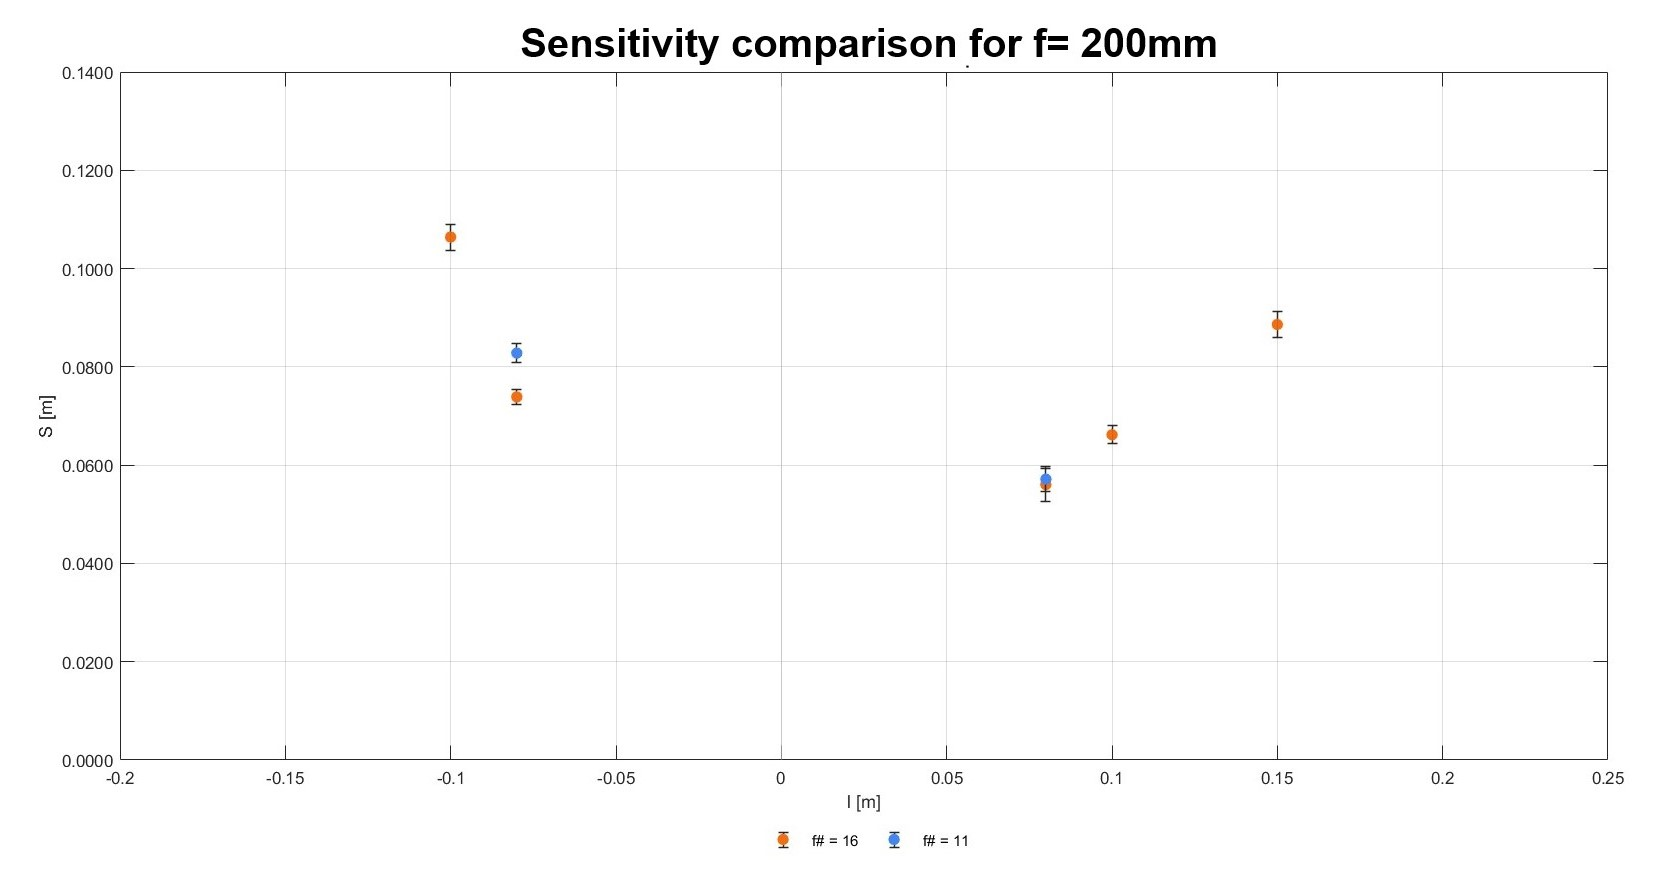
\includegraphics[width=\textwidth]{figures/S vs l experimental.jpg}
        \caption{}
        \label{fig: S vs l experimental}
    \end{subfigure}
    \hfill
    \begin{subfigure}[b]{0.49\textwidth}
        \centering
        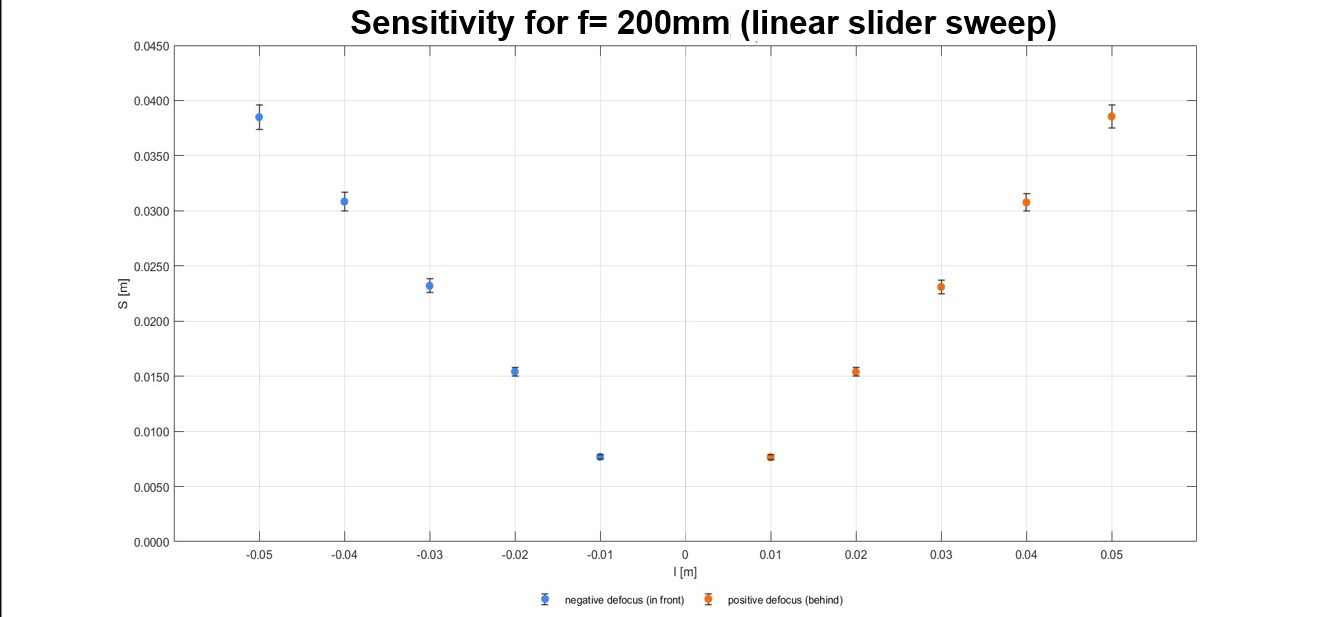
\includegraphics[width=\textwidth]{figures/S vs l slider experiment.jpg}
        \caption{}
        \label{fig: S vs l slider experiment}
    \end{subfigure}
    \caption{Sensitivity versus defocus distance for a camera lens of $f = 200$ mm. (a) Points obtained with $f_\# = 11$ and $f_\# = 16$ for an enforced $L_{FoV_{obj}} = 17$ mm. (b) Points obtained in the slider experiment, with a fixed measured magnification of $M_{ag} = 0.746$}
    \label{fig: S vs l experiments}
\end{figure}

Figure \ref{fig: S vs l experimental} replicates one of the predictions of Chapter \ref{chapter: methodology}, where a higher sensitivity was obtained for the same defocus distance if a negative defocus was chosen instead of its positive one. It is also worth noting that all points were obtained with the same field of view of the object. Therefore, a higher sensitivity and magnification are achieved while capturing the same area of the object. Although the resolution has not been measured in this case, it is also to be expected through Equation \ref{equation: S over smin} that the spatial resolution trade-off is improved by this increase in magnification. This figure effectively compares the performance of SBOS with BOS, answering one of the research questions posed in Chapter \ref{chapter: introduction}.


% REVIEW: the last two sentences say the same thing. The second one says "shorter focal length", but f was fixed; the quantity that changes is the focal distance d_f. "More powerful" is vague, consider "more sensitive".
Points 10 to 20 of Tables \ref{tab: angled glass displacement results} and \ref{tab: sensitivity comparison} show the results of the experiment where the angled glass was positioned in a linear slider with a fixed magnification and only the defocus position was changed. Figure \ref{fig: S vs l slider experiment} plots the resulting sensitivity against the defocusing distance. The points are symmetric around the Y-axis, which means that the mechanism that makes a negative defocus configuration more powerful than its positive counterpart is not the negative distance per se but the increased magnification that comes with a shorter focal distance to the camera. Therefore, the mechanism making negative defocus more sensitive than standard defocus is the higher magnification that comes with a shorter focal length.

% REVIEW: Chapter 4 presents Equation 4.9 as the minimum speckle size, here it is the predicted average size. The discrepancy is not only "at some points": every point exceeds the prediction by at least a factor of four.
Section \ref{section: Angled Glass Experiment} mentioned a discrepancy between the predicted average speckle size obtained through the Rayleigh diffraction limit and the ones obtained experimentally and computed using Hamarová's method \cite{Hamarova2016}. Table \ref{tab: angled glass speckle results} displays both quantities side by side together with the $f_\#$ and $M_{ag}$ used at each point. The $\Delta s$ deviation shows that at some points the discrepancy exceeds the theoretical value several times. Speckle formation is an intrinsically random phenomenon, described by complex physics \cite{Goodman2020, NikitaFominBook, Cloud2007}, so it is not exactly clear what is precisely the root of this difference. Nevertheless, the data gives some clues on what could be improved.

% REVIEW: this section finds that the speckle size follows M_ag and ignores f#, while Section 6.2 finds the opposite. Consider one paragraph that names both regimes. The mechanism is also stated three ways: imaged phase cells at the diffuser (here), laser diffraction limited in the diffuser (section summary) and small beam on the diffuser (Section 6.2). Pick one.
It seems that the f-stop number did not influence the average speckle size obtained experimentally. This becomes evident from observing points 4 and 8--10. In these points, the $f_\#$ ranges from 4 to 16 whereas $\Delta s$ stays within 12.35 px to 12.94 px. In contrast, changes in magnification were observed to have an effect in the experimental average speckle size considerably. From points 1--4 the $f_\#$ is fixed and $M_{ag}$ changes from 0.671 to 1.045, displaying $\Delta s$ from 12.74 px to 21.21 px. These factors contradict the Rayleigh equation for subjective speckles where its size is only dependent on the light's wavelength, imaging lens $f_\#$ and $M_{ag}$. The independence to the aperture size indicates that the interference pattern is not being created at the lens pupil as it should \cite{Goodman2020}. The magnification effect, in turn, means that the speckle is behaving like an imaged object. These factors lead to the belief that the pattern did not form a Rayleigh distribution at the lens pupil, rather what is being imaged are just the phase cells illuminated at the diffuser.

%This is a stretch from Goodman "If the diffuser overfills the projection lens, then each projector resolution cell undergoes a random walk of amplitudes scattered from the diffuser, resulting in an independent Rayleigh-distributed amplitude and uniformly distributed phase for each of such projection-lens resolution cells incident on the screen."


\begin{table}[htbp]
    \centering

% REVIEW: Delta s_th was computed with the design magnification (point 1: 3.72 px with M_th = 0.956, 3.80 px with M_exp = 1.002), but the column shows M_ag_exp. Recompute or state it in the caption.
    \caption{Speckle sizes measured during the angled glass campaign, for the configurations of Table \ref{tab: angled glass test matrix}. $M_{ag_{exp}}$ is the magnification measured with the calibration plate, $\Delta s_{th}$ the size predicted by the Rayleigh limit of Equation \ref{equation: Rayleigh Limit} and $\Delta s_{exp}$ the size returned by the one-dimensional autocorrelation method of Hamarová et al. \cite{Hamarova2016}, taken as the lag at which the normalised autocorrelation of intensity falls to $1/e$. The last column is the difference between the two. Points 11 to 20 share the optical layout of point 10, so their predicted and measured sizes are identical and have been omitted.}
    \label{tab: angled glass speckle results}
    \begin{tabular}{lrrrrr}
        \toprule
        Point & $f_\#$ & $M_{ag_{exp}}$ &  $\Delta s_{th}$ & $\Delta s_{exp}$ & $\Delta s$ dev. \\
              & [--] & [--] & [px] & [px] & [px] \\
        \midrule
         1 & 16.00 & 1.002 &   3.72 &  20.30 & $+16.58$ \\
         2 & 16.00 & 0.688 &   3.15 &  13.05 & $+9.90$ \\
         3 & 16.00 & 1.045 &   3.90 &  21.21 & $+17.31$ \\
         4 & 16.00 & 0.671 &   3.12 &  12.74 & $+9.62$ \\
         5 & 11.31 & 1.043 &   2.74 &  20.78 & $+18.04$ \\
         6 & 11.31 & 0.718 &   2.27 &  14.12 & $+11.85$ \\
         7 & 11.31 & 1.054 &   3.02 &  25.32 & $+22.30$ \\
         8 &  4.00 & 0.572 &   0.75 &  12.35 & $+11.60$ \\
         9 & 16.00 & 0.640 &   3.06 &  12.65 & $+9.59$ \\
        10 &  8.00 & 0.746 &   1.65 &  12.94 & $+11.29$ \\
        \bottomrule
    \end{tabular}
\end{table}


% REVIEW: the mechanism given here (laser diffraction limited in the diffuser) differs from the one in the speckle paragraph above and from the one in Section 6.2.
In this section, the results, errors and associated uncertainties of the angled glass experiments have been presented. The two plots constructed with the data collected permit answering one of this thesis' research questions and infer the mechanism that explains the advantage in performance of SBOS in comparison to BOS. Nevertheless, there was one prediction from theory that could not be verified in this experimental campaign: the average speckle size given by Rayleigh diffraction. The speckles obtained were considerably larger and did not change with the lens f-stop number, which led to the belief that the laser ray was becoming diffraction limited in the ground glass diffuser instead of the lens pupil. Another experimental campaign was envisioned to try and obtain a finer speckle pattern before the implementation of SBOS to a wind-tunnel application.


\section{Speckle Pattern Investigation Results}
\label{section: Speckle Pattern Experiment Results}

Faced with the difficulties in creating a satisfactory speckle pattern in the first experimental campaign, the second experiment aimed to investigate ways to generate a finer average speckle size, try to produce a Rayleigh distribution at the lens pupil and compare the implications of generating a speckle through direct diffusion or by projecting the laser into a surface. Table \ref{tab: speckle results} presents the data obtained with the experimental setups described in Section \ref{section: Speckle Pattern Investigation} with the conditions displayed in Tables \ref{tab: speckle investigation matrix} for direct speckles and \ref{tab: projected speckle matrix} for projected speckles. This section discusses the computed average speckle sizes obtained at each point, the deviation from the Rayleigh limit of Equation \ref{equation: Rayleigh Limit} and a quantification of the experiment's associated uncertainties.


%The main goals were to better understand the creation of a finer speckle pattern assess how the average speckle size correlates to the Rayleigh limit of Equation \ref{equation: Rayleigh Limit} and also compare the generation of speckles through direct ground glass diffusion and by projecting the laser into a surface.

\begin{table}[htbp]
    \centering
% REVIEW: Delta s_th of points 1-13 and 29-31 uses the design magnification (point 29: 0.67 px with M = 0.417, 0.69 px with M_exp = 0.457). The caption says M_ag_exp was measured with the calibration plate, but the magnification sweep figure says points 14-28 used the lens distance marks, and that uncertainty is not in the budget.
    \caption{Speckle sizes measured during the experimental campaign, using the optical configurations of Table \ref{tab: speckle investigation matrix}. $M_{ag_{exp}}$ is the magnification measured with the calibration plate, $\Delta s_{th}$ is the size predicted by the Rayleigh limit and $\Delta s_{exp}$ is the estimated experimental size, reported both by the DaVis function and by the method of Hamarová et al. \cite{Hamarova2016}. The deviation columns give the difference of each measurement from the prediction. The column $u_{tot}$ is the combined standard uncertainty of $\Delta s_{exp}$. Points 1 to 13 vary the aperture and the ground glass distance, whereas points 14 to 28 hold both fixed and sweep the magnification. Points 29 to 31 were obtained with projected speckles, using the parameters of Table \ref{tab: projected speckle matrix}.}
    \label{tab: speckle results}
    \begin{tabular}{lrrrrrrrrr}
        \toprule
        Point & $f_\#$ & $d_{GG}$ & $M_{ag_{exp}}$ & $\Delta s_{th}$ & \multicolumn{3}{c}{Hamarová} & \multicolumn{2}{c}{DaVis} \\
        \cmidrule(lr){6-8} \cmidrule(lr){9-10}
              & [--] & [mm] & [--] & [px] & $\Delta s_{exp}$ & $\Delta s$ dev. & $u_{tot}$ & $\Delta s_{exp}$ & $\Delta s$ dev. \\
              &      &      &      &      & [px] & [px] & [\%] & [px] & [px] \\
        \midrule
         1 &  4.00 &  740 & 0.964 &  0.92 &  1.74 &  $+0.82$ &  6.35 &   1.20 &  $+0.28$ \\
         2 & 11.31 &  740 & 0.964 &  2.59 &  2.73 &  $+0.14$ &  1.50 &   1.48 &  $-1.11$ \\
         3 & 22.63 &  740 & 0.964 &  5.19 &  3.83 &  $-1.36$ & 11.45 &   2.00 &  $-3.19$ \\
         4 &  4.00 &  740 & 0.296 &  0.61 &  1.62 &  $+1.02$ &  2.62 &   1.19 &  $+0.59$ \\
         5 & 11.31 &  740 & 0.296 &  1.71 &  2.71 &  $+1.00$ &  7.11 &   1.56 &  $-0.15$ \\
         6 & 22.63 &  740 & 0.296 &  3.42 &  3.81 &  $+0.39$ &  4.87 &   2.04 &  $-1.39$ \\
         7 & 11.31 &  450 & 0.296 &  1.71 &  2.29 &  $+0.58$ &  6.60 &   1.35 &  $-0.36$ \\
         8 & 11.31 &  280 & 0.296 &  1.71 &  2.45 &  $+0.74$ &  2.87 &   1.40 &  $-0.31$ \\
         9 & 11.31 &  190 & 0.296 &  1.71 &  2.91 &  $+1.20$ &  2.79 &   1.59 &  $-0.12$ \\
        10 & 11.31 &  100 & 0.296 &  1.71 &  4.59 &  $+2.88$ &  3.12 & failed &       -- \\
        11 &  4.00 &  300 & 0.877 &  0.88 &  2.42 &  $+1.54$ &  1.50 &   1.45 &  $+0.57$ \\
        12 & 11.31 &  300 & 0.877 &  2.49 &  2.98 &  $+0.49$ &  1.50 &   1.67 &  $-0.82$ \\
        13 & 22.63 &  300 & 0.877 &  4.97 &  4.15 &  $-0.83$ &  1.55 &   2.41 &  $-2.56$ \\
        \midrule
        14 & 22.63 &  300 & 1.000 &  5.37 &  3.05 &  $-2.33$ &  1.52 &   1.81 &  $-3.57$ \\
        15 & 22.63 &  300 & 0.909 &  5.13 &  3.14 &  $-1.99$ &  1.50 &   1.76 &  $-3.38$ \\
        16 & 22.63 &  300 & 0.800 &  4.84 &  3.26 &  $-1.58$ &  1.50 &   1.86 &  $-2.98$ \\
        17 & 22.63 &  300 & 0.667 &  4.48 &  2.66 &  $-1.81$ &  6.43 &   1.60 &  $-2.88$ \\
        18 & 22.63 &  300 & 0.571 &  4.22 &  2.80 &  $-1.42$ &  4.78 &   1.65 &  $-2.57$ \\
        19 & 22.63 &  300 & 0.500 &  4.03 &  2.39 &  $-1.64$ &  2.80 &   1.47 &  $-2.56$ \\
        20 & 22.63 &  300 & 0.400 &  3.76 &  3.60 &  $-0.16$ &  2.39 &   1.68 &  $-2.08$ \\
        21 & 22.63 &  300 & 0.333 &  3.58 &  2.16 &  $-1.42$ &  4.13 &   1.42 &  $-2.16$ \\
        22 & 22.63 &  300 & 0.286 &  3.46 &  2.38 &  $-1.07$ &  3.39 &   1.48 &  $-1.97$ \\
        23 & 22.63 &  300 & 0.222 &  3.28 &  2.53 &  $-0.76$ &  4.66 &   1.59 &  $-1.70$ \\
        24 & 22.63 &  300 & 0.167 &  3.13 &  2.88 &  $-0.25$ &  3.33 &   1.74 &  $-1.39$ \\
        25 & 22.63 &  300 & 0.118 &  3.00 &  3.06 &  $+0.06$ &  3.42 &   1.91 &  $-1.09$ \\
        26 & 22.63 &  300 & 0.074 &  2.89 &  2.72 &  $-0.17$ &  3.05 &   1.65 &  $-1.23$ \\
        27 & 22.63 &  300 & 0.054 &  2.83 &  2.76 &  $-0.07$ &  1.82 &   1.71 &  $-1.12$ \\
        28 & 22.63 &  300 & 0.035 &  2.78 &  3.09 &  $+0.31$ &  5.47 &   1.87 &  $-0.91$ \\
        \midrule
        29 &  4.00 &  300 & 0.457 &  0.67 &  1.59 &  $+0.92$ &  1.54 &   1.22 &  $+0.55$ \\
        30 & 11.31 &  300 & 0.457 &  1.90 &  2.21 &  $+0.31$ &  1.80 &   1.44 &  $-0.46$ \\
        31 & 22.63 &  300 & 0.457 &  3.81 &  3.61 &  $-0.20$ &  2.08 &   2.09 &  $-1.72$ \\
        \bottomrule
    \end{tabular}
\end{table}

Table \ref{tab: speckle results} and Figure \ref{fig: speckle size per point} show the average speckle size obtained experimentally for each point. They present the experimental speckle sizes obtained using DaVis' function together with the ones computed through Hamarová et al.'s autocorrelation method \cite{Hamarova2016}. A comparison between the two methods yielded some differences in magnitudes, with DaVis ranging from 1.19 to 2.41 px, while the autocorrelation spans from 1.59 to 4.59 px. Despite this difference, both methods reproduce the same trends reliably as shown by Figure \ref{fig: speckle size per point}. Since it is known how the estimator of Hamarová et al. works, contrary to the DaVis estimator, and both reproduce the same behavior, from now on the discussion will focus only on the results obtained with the autocorrelation method.

\begin{figure}[htbp]
    \centering
    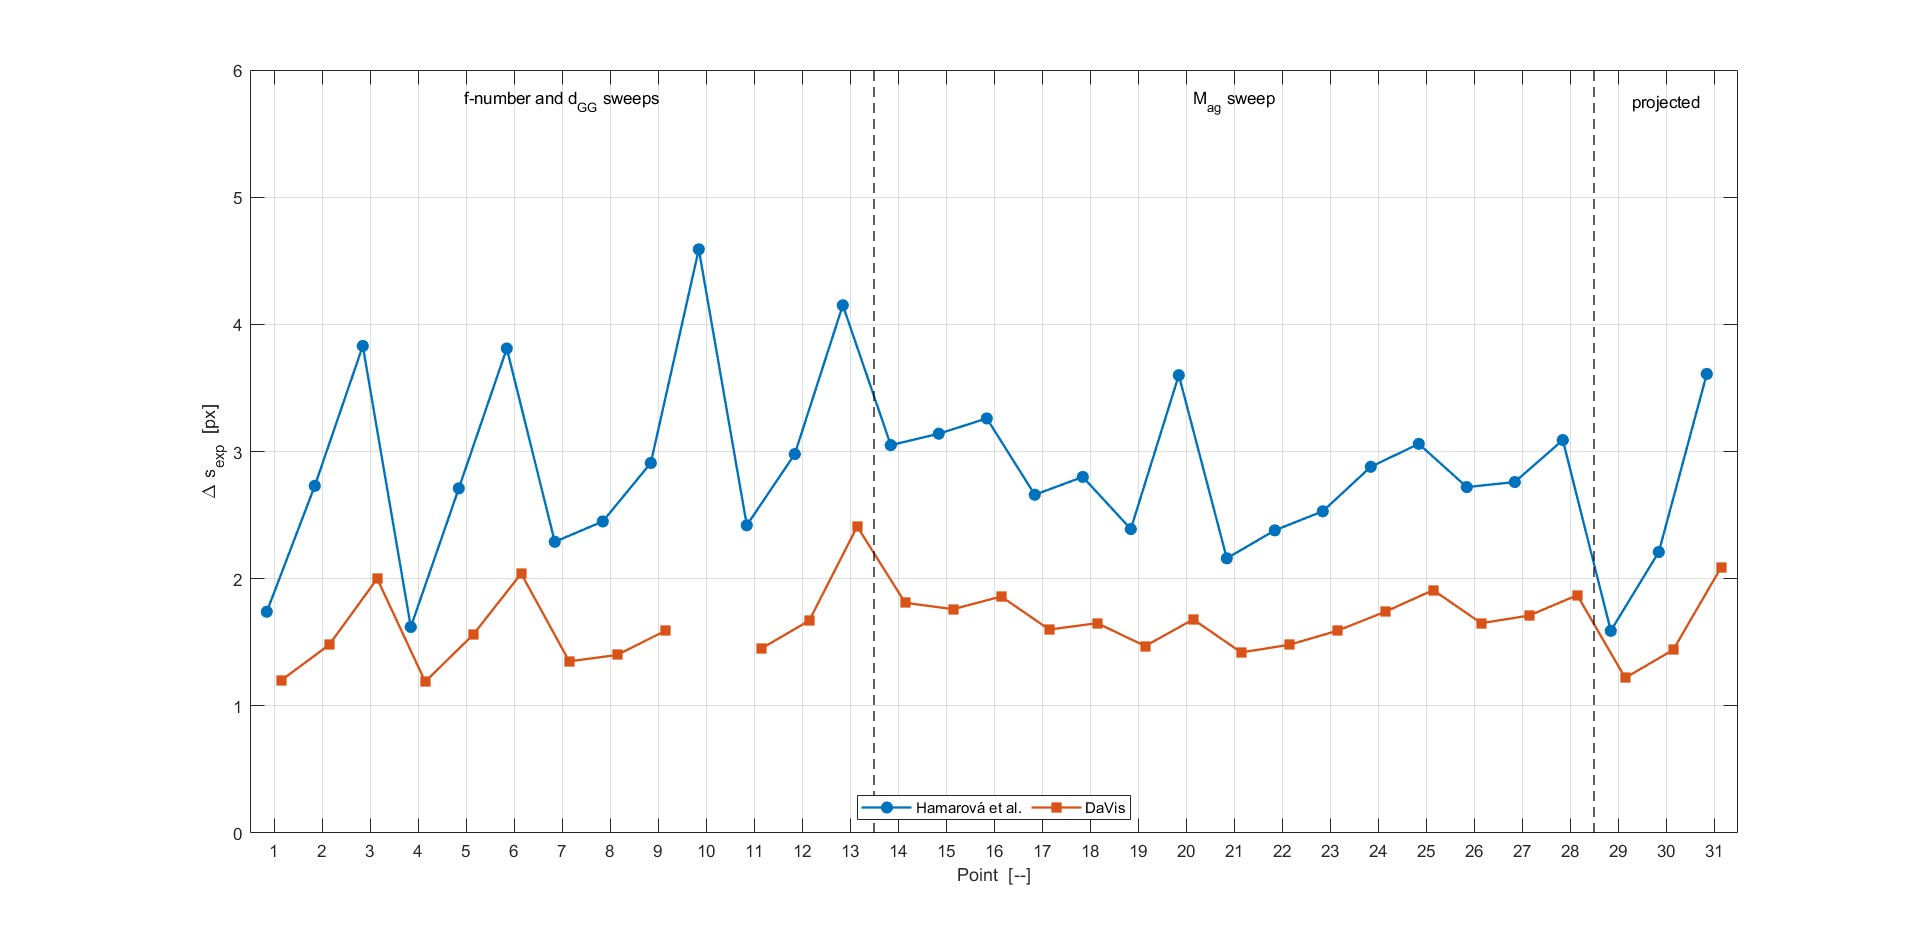
\includegraphics[width=\textwidth]{figures/speckle size per point.jpg}
    \caption{Average speckle size of every point of Table \ref{tab: speckle results}, computed with the autocorrelation method of Hamarová et al. \cite{Hamarova2016} and with the DaVis function. The dashed lines separate the $f_\#$ and $d_{GG}$ sweeps, the magnification sweep and the projected speckle points. DaVis returned no value for point 10}
    \label{fig: speckle size per point}
\end{figure}

% REVIEW: the deviations are in px while u_tot is in percent, so "vastly surpasses" compares different units, and it does not hold at every point (point 25: 0.06 px on 3.00 px is 2 percent, below u_tot = 3.42 percent). The magnification uncertainty "within 5% for a 10% deviation" has no budget in the thesis.
Regarding the Rayleigh limit reproduction, it is possible to see that the results are much more similar to the predicted values in order of magnitude if compared to the ones presented previously in Table \ref{tab: angled glass speckle results}. The deviations now span from 0.06 px to a maximum of 2.88 px, instead of 9.59 to 22.30 px from before. Nevertheless, the relative error is still large overall, with the worst results at the points with subpixel speckles and close to 5 px. The error also vastly surpasses the uncertainty associated with magnification, which stayed within 5\% for a 10\% deviation in $M_{ag}$, and post-processing, which had a maximum of 11.45\%. Regardless, the data obtained provides a better fit to the Rayleigh diffraction prediction, showing that the equation can be used as a rough preliminary estimator of the speckle size. The results also allow for the identification of useful trends and comparisons in speckle production, as will be shown.

% REVIEW: "direct speckles provide more intensity, which allows for lower exposures" is not supported by data in this chapter. Add a measurement or a citation.
Points 29 to 31 of Table \ref{tab: speckle results} were obtained with projected speckles. Compared to direct speckles, the projected speckles show a similar deviation to theory and an overall smaller speckle size, which is hinted by Figure \ref{fig: speckle f-number sweep}. The results are too similar to the direct speckle approach to discriminate which method to use based on speckle size. Therefore, the trade-off on how to create the speckle pattern depends more on practical considerations than on its speckle characteristics. Projected speckles might be preferable in applications where only one optical access is available; where powerful lasers are being used that could damage the camera or when the double-pass method of Meier \& Rösgen \cite{Meier&Roesgen2013} needs to be used for increased sensitivity. Direct speckles, on the other hand, provide more intensity, which allows for lower exposures, and might be preferable when a see-through optical access is available. 

%However, it might be more vulnerable to vibrations and decorrelation \cite{Buhlmann2020}, specially in cases where the background is very close to the test-section.

% The vulnerability to decorrelation mentioned in chapter 3 doesn't seem to be an exclusive issue to projected speckle but transversal to both configurations. It is caused when the diffusor is submitted to some degree of motion or vibration, specially when positioned very close to the test section. 

% REVIEW: the text and Table 6.8 describe the budget differently. Half-width: the standard deviation that minimizes the tail beyond 60 px (text) vs the range of widths within the noise floor (caption). Estimator term: the 1.5 percent reported by Hamarova (text) vs the spread between three estimators (caption). "As a consequence" does not follow from the previous sentence.
To better judge the deviation of the experiment, an uncertainty budget was constructed to compute the total uncertainties. They are displayed for each experimental point in Table \ref{tab: speckle results}. This total uncertainty corresponds to the ones obtained for the implementation of Hamarová et al.'s method and is reported in Table \ref{tab: speckle size uncertainty}. In their paper, the researchers reported an uncertainty of 1.5\% associated with their estimator. As a consequence, the budget is dominated by the Gaussian filter implemented. The Gaussian standard deviation was taken as a parameter and varied such that the tail of the autocorrelation function result after 60 px was minimized. The half-width of the method is, therefore, the achieved standard deviation and its individual uncertainty, assuming a rectangular distribution, is $u = a / \sqrt{3}$. The contribution is $u$ times the sensitivity coefficient. In the last row, the combined figure of the post-processing uncertainty can be found.

\begin{table}[htbp]
    \centering
    \caption{Uncertainty budget for the average speckle size obtained by the autocorrelation method. The flattening filter width is not measured with an instrument; it is selected by driving the tail of the autocorrelation to zero, so its half-width $a$ is the range of widths for which that tail remains within its noise floor, taken as $1/\sqrt{N_s}$ for a frame holding $N_s$ speckles. As in Table \ref{tab: angled glass uncertainty}, the width is treated as a rectangular distribution so that $u = a/\sqrt{3}$ \cite{JCGM2008}, and the contribution $c_\sigma$ is the sensitivity $\partial \Delta s_{exp} / \partial \sigma$, obtained by re-evaluating the speckle size one pixel either side of the selected width, multiplied by $u$. The estimator contribution is the spread between the two-dimensional, the average one-dimensional and the long vector estimators reported by Hamarová et al. \cite{Hamarova2016}. Both terms vary per point, so their range over the 31 points is given here and the totals are listed per point in Table \ref{tab: speckle results}.}
    \label{tab: speckle size uncertainty}
    \begin{tabular}{llrrr}
        \toprule
        Source & Instrument & $a$ & $u$ & Contribution $c_i$ [\%] \\
        \midrule
        Filter width $\sigma$      & Tail criterion & 2.0--67.0 px & 1.2--38.7 px & 0.06--11.36 \\
        Estimator choice           & Literature     & --           & 1.5 \%       & 1.50 \\
        \midrule
        Combined, $u_{\Delta s} = \sqrt{c_\sigma^2 + c_{est}^2}$ &  &  &  & 1.50--11.45 \\
        \bottomrule
    \end{tabular}
\end{table}

%Maybe this paragraph could be split into mag, aperture, d_GG and projected
% REVIEW: long paragraph, consider splitting it into aperture, magnification, d_GG and projected speckles. The magnification insensitivity found here is the opposite of Section 6.1 and needs to be reconciled.
Now that the error and uncertainties of the results have been discussed, the data can be plotted to better understand its behavior, such as f-stop dependency. The various $f_\#$ sweeps made during the experimental campaign allow the evaluation of whether the interference waves became diffraction limited at the pupil. Figure \ref{fig: speckle f-number sweep} shows the trend of average speckle size with f-stop number for four different configurations. All lines follow the characteristic increasing trend of a developed subjective speckle, which follows Equation \ref{equation: Rayleigh Limit}, and signals that the interference front is becoming diffraction limited at the lens pupil \cite{Goodman2020}. The red and yellow lines both share the same $d_{GG}$, which makes them viable for direct comparison. It appears that the increased magnification of the red line caused practically no effect in the average speckle size, displaying almost the same values as the yellow line. The same insensitivity to magnification was also experienced through points 14--28 shown in Figure \ref{fig: speckle magnification sweep}. Looking at the purple line compared to the latter two, it appears that the different $d_{GG}$ introduced some difference in the speckle size, with the purple exceeding the red by 0.68, 0.25 and 0.32 px for $f_\#$ = 4, 11.31 and 22.63, respectively, although the difference is only subpixel. In green, the projected speckle trend can also be analyzed, and it demonstrates that projected speckles are generally smaller, presenting smaller speckles even than the yellow line, which has a lower magnification than green. The figure shows some promising trends as there is a clear dependence on $f_\#$ and it indicates a tendency of projected speckles to be smaller than direct ones. However, it also shows an insensitivity to the optical magnification, contradicting Equation \ref{equation: Rayleigh Limit}, and the effect of $d_{GG}$ which will be further discussed next.

\begin{figure}[htbp]
    \centering
    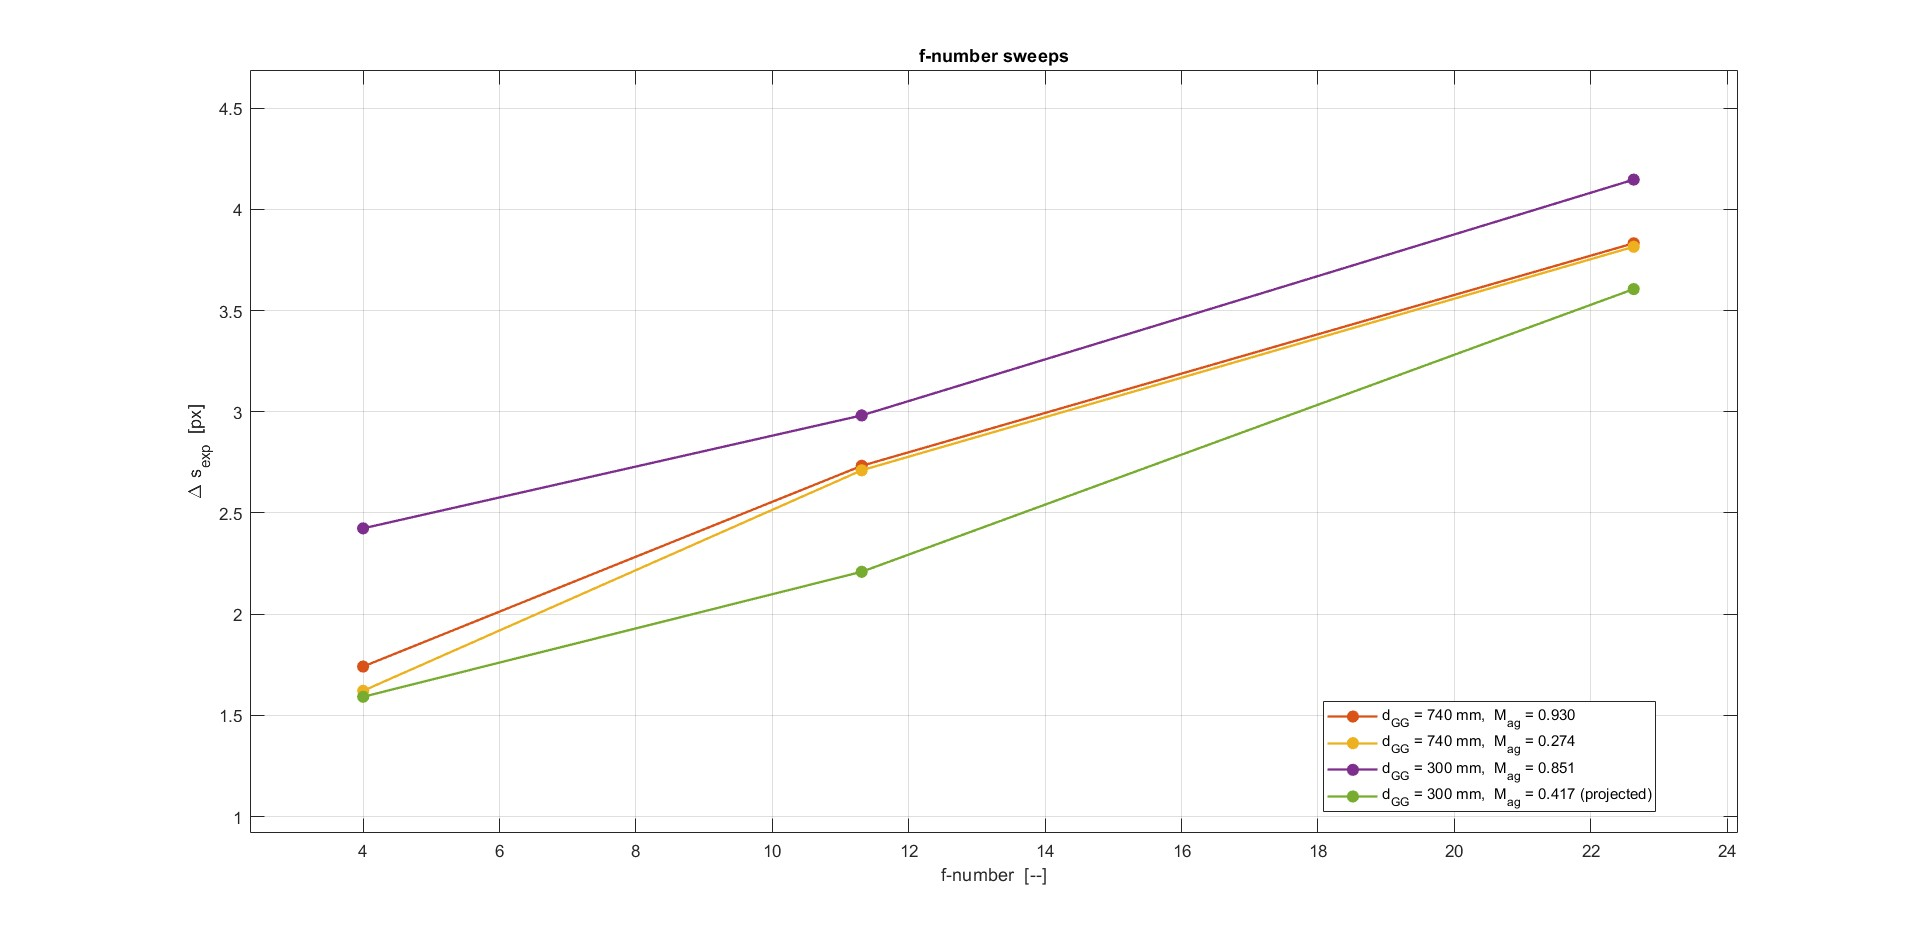
\includegraphics[width=\textwidth]{figures/speckle exp f-number sweep.jpg}
    \caption{Average speckle size versus f-stop number for the four aperture sweeps of the speckle investigation campaign. The red and yellow lines correspond to points 1--3 and 4--6, which share $d_{GG} = 740$ mm at two different magnifications. The purple line corresponds to points 11--13, acquired at $d_{GG} = 300$ mm, and the green line to points 29--31, obtained with projected speckles at the same $d_{GG}$}
    \label{fig: speckle f-number sweep}
\end{figure}


% REVIEW: "beam ratio of 0.25" is not defined. The literature argument is from silence ("does not mention the effect"). The final recommendation generalizes from five points at one f# and one M_ag. The mechanism should match the one used in Section 6.1.
Since the beam was expanded through a convergent lens, the distance between that lens and the ground glass diffuser is a proxy for the beam diameter, therefore, it is possible to verify the influence of the beam diameter in the speckle generation by plotting the points where only $d_{GG}$ was varied. Figure \ref{fig: speckle dGG sweep} shows that the average speckle size remains consistent for high $d_{GG}$, as it varies from 2.91 px at 190 mm, dips to 2.29 px at 450 mm and goes to 2.71 px at 740 mm. This variation is consistent with the findings of Figure \ref{fig: speckle f-number sweep}. It demonstrates that $d_{GG}$ can increase the speckle size but for large distances the spread is practically subpixel. However, the figure also shows a spike at low $d_{GG}$ when the beam diameter is small, reaching 4.59 px at 100 mm with beam ratio of 0.25. The DaVis function failed to compute a value for this point, as the illuminated envelope was too small and the speckles too large. The effect can be better visualized through Figure \ref{fig: speckle patterns dGG} which displays side-by-side the captured speckle patterns for points 5, 8 and 10 respectively. This data supports the hypothesis that the larger speckle size in the angled glass experiment was caused by the small diameter of the laser when it hit the 1.27 cm ground glass diffuser. The fact that the speckle size changed less for larger distances is also backed up by the literature, which does not mention the effect of the laser diameter in the speckle generation. In addition, it means that, when designing the laser optical setup, an experimentalist must only worry about expanding the laser beam to fill the desired field of view.

\begin{figure}[htbp]
    \centering
    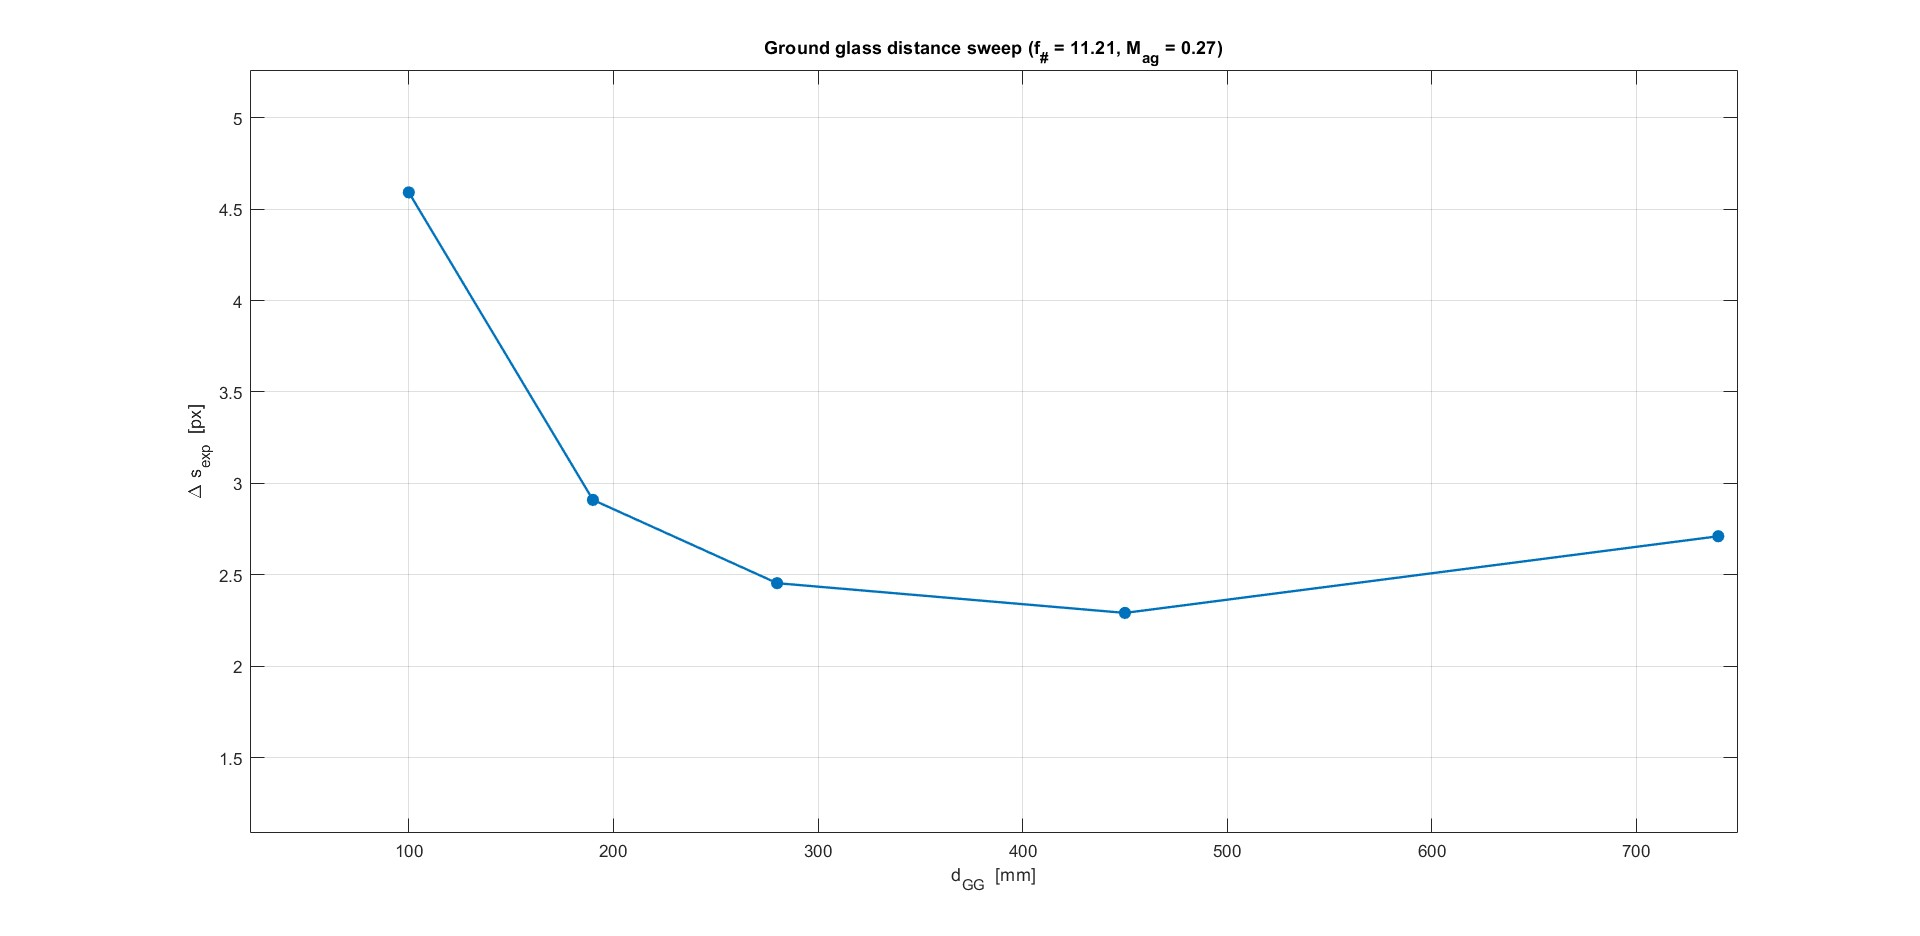
\includegraphics[width=\textwidth]{figures/Speckle d_GG Sweep.jpg}
    \caption{Average speckle size versus the distance between the beam expander lens and the ground glass diffuser, for points 5 and 7--10 of Table \ref{tab: speckle results}, all acquired at $f_\# = 11.31$ and $M_{ag_{exp}} = 0.296$}
    \label{fig: speckle dGG sweep}
\end{figure}

\begin{figure}[htbp]
    \centering
    \begin{subfigure}[b]{0.32\textwidth}
        \centering
        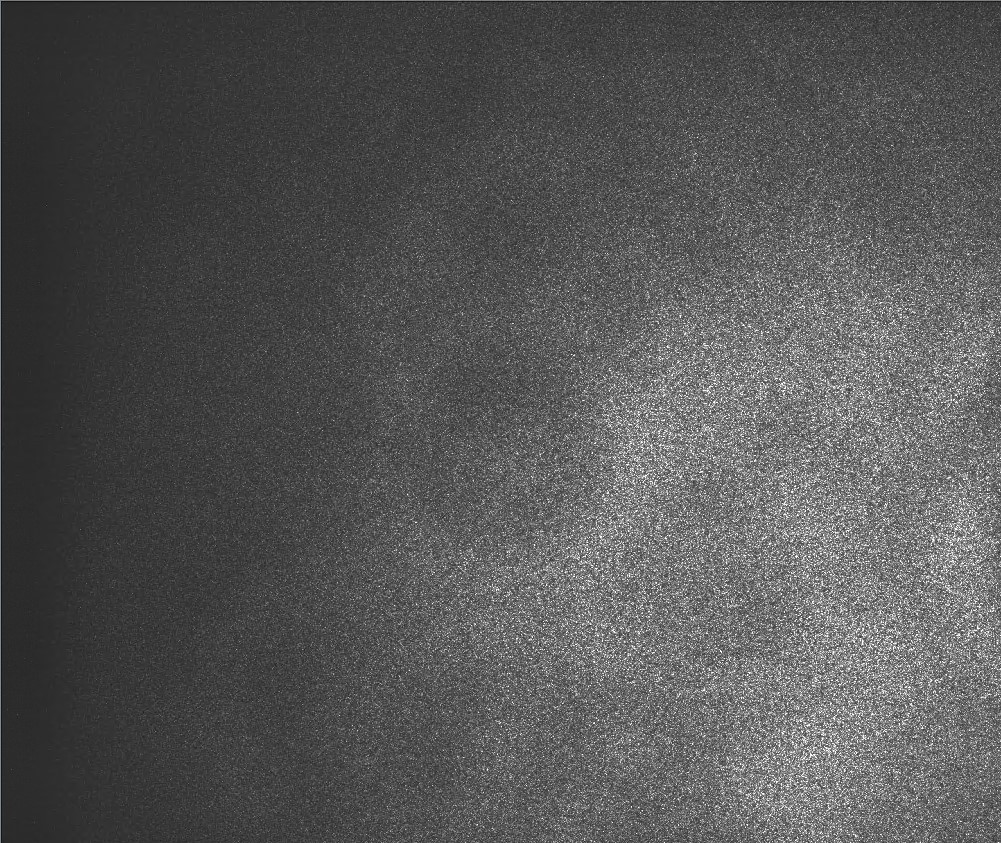
\includegraphics[width=\textwidth]{figures/Speckle pattern point 5.jpg}
        \caption{Point 5, $d_{GG} = 740$ mm}
        \label{fig: speckle pattern point 5}
    \end{subfigure}
    \hfill
    \begin{subfigure}[b]{0.32\textwidth}
        \centering
        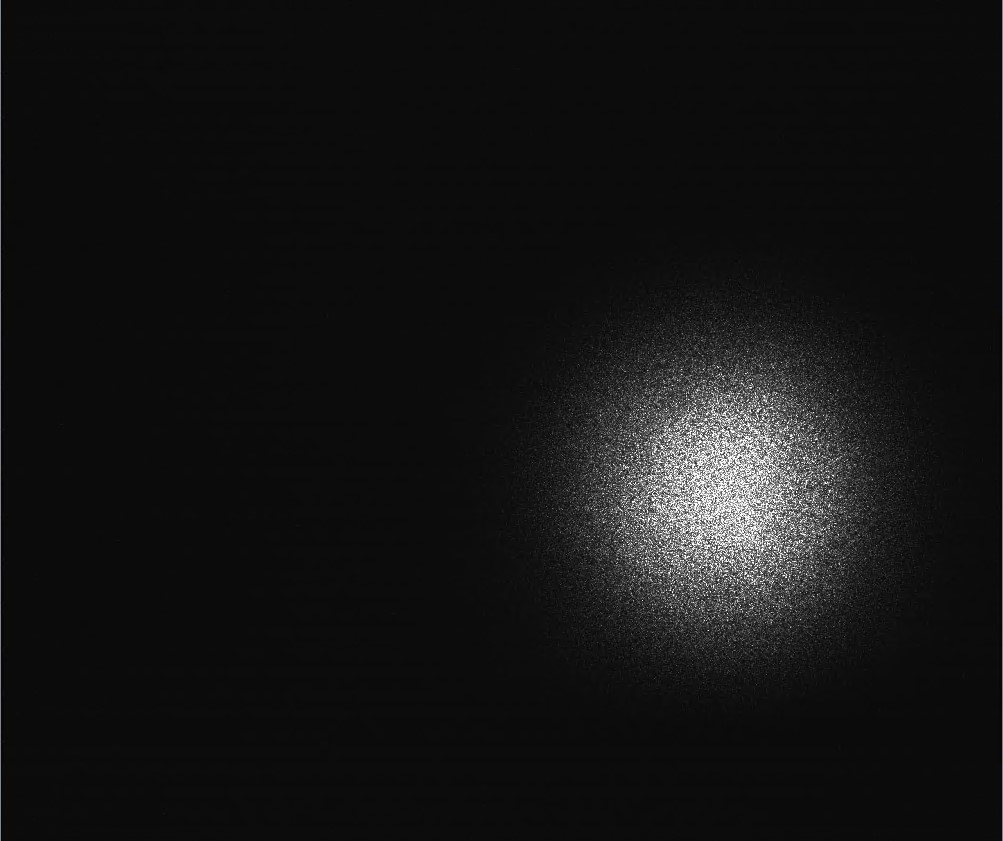
\includegraphics[width=\textwidth]{figures/Speckle pattern point 8.jpg}
        \caption{Point 8, $d_{GG} = 280$ mm}
        \label{fig: speckle pattern point 8}
    \end{subfigure}
    \hfill
    \begin{subfigure}[b]{0.32\textwidth}
        \centering
        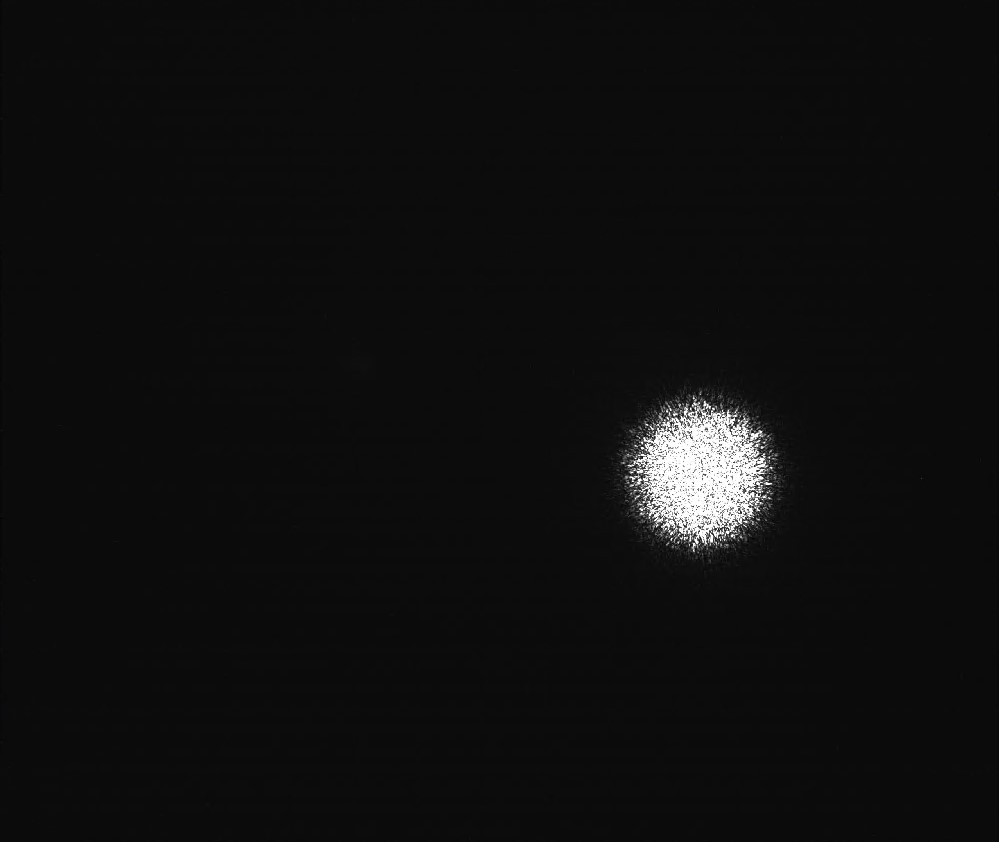
\includegraphics[width=\textwidth]{figures/Speckle pattern point 10.jpg}
        \caption{Point 10, $d_{GG} = 100$ mm}
        \label{fig: speckle pattern point 10}
    \end{subfigure}
    \caption{Raw speckle patterns captured at $f_\# = 11.31$ and $M_{ag_{exp}} = 0.296$ for three distances between the beam expander lens and the ground glass diffuser. As $d_{GG}$ decreases, the illuminated area on the diffuser shrinks and the speckle pattern contracts from filling the sensor to a small bright spot}
    \label{fig: speckle patterns dGG}
\end{figure}


To better assess the effect of optical magnification in the speckle generation process, a sweep of the focal distance was conducted through points 14--28 and is shown in Figure \ref{fig: speckle magnification sweep}. It is worth mentioning that the magnification value of these points is less accurate than the others, as the focal distance was obtained through the distance marks of the camera lens. Nevertheless, the figure shows, for a different $d_{GG}$, the same speckle size insensitivity to optical magnification that was identified in Figure \ref{fig: speckle f-number sweep}. That effectively contradicts the Rayleigh diffraction limit equation and reduces the number of control variables an experimentalist would have when designing the experimental setup.

\begin{figure}[htbp]
    \centering
    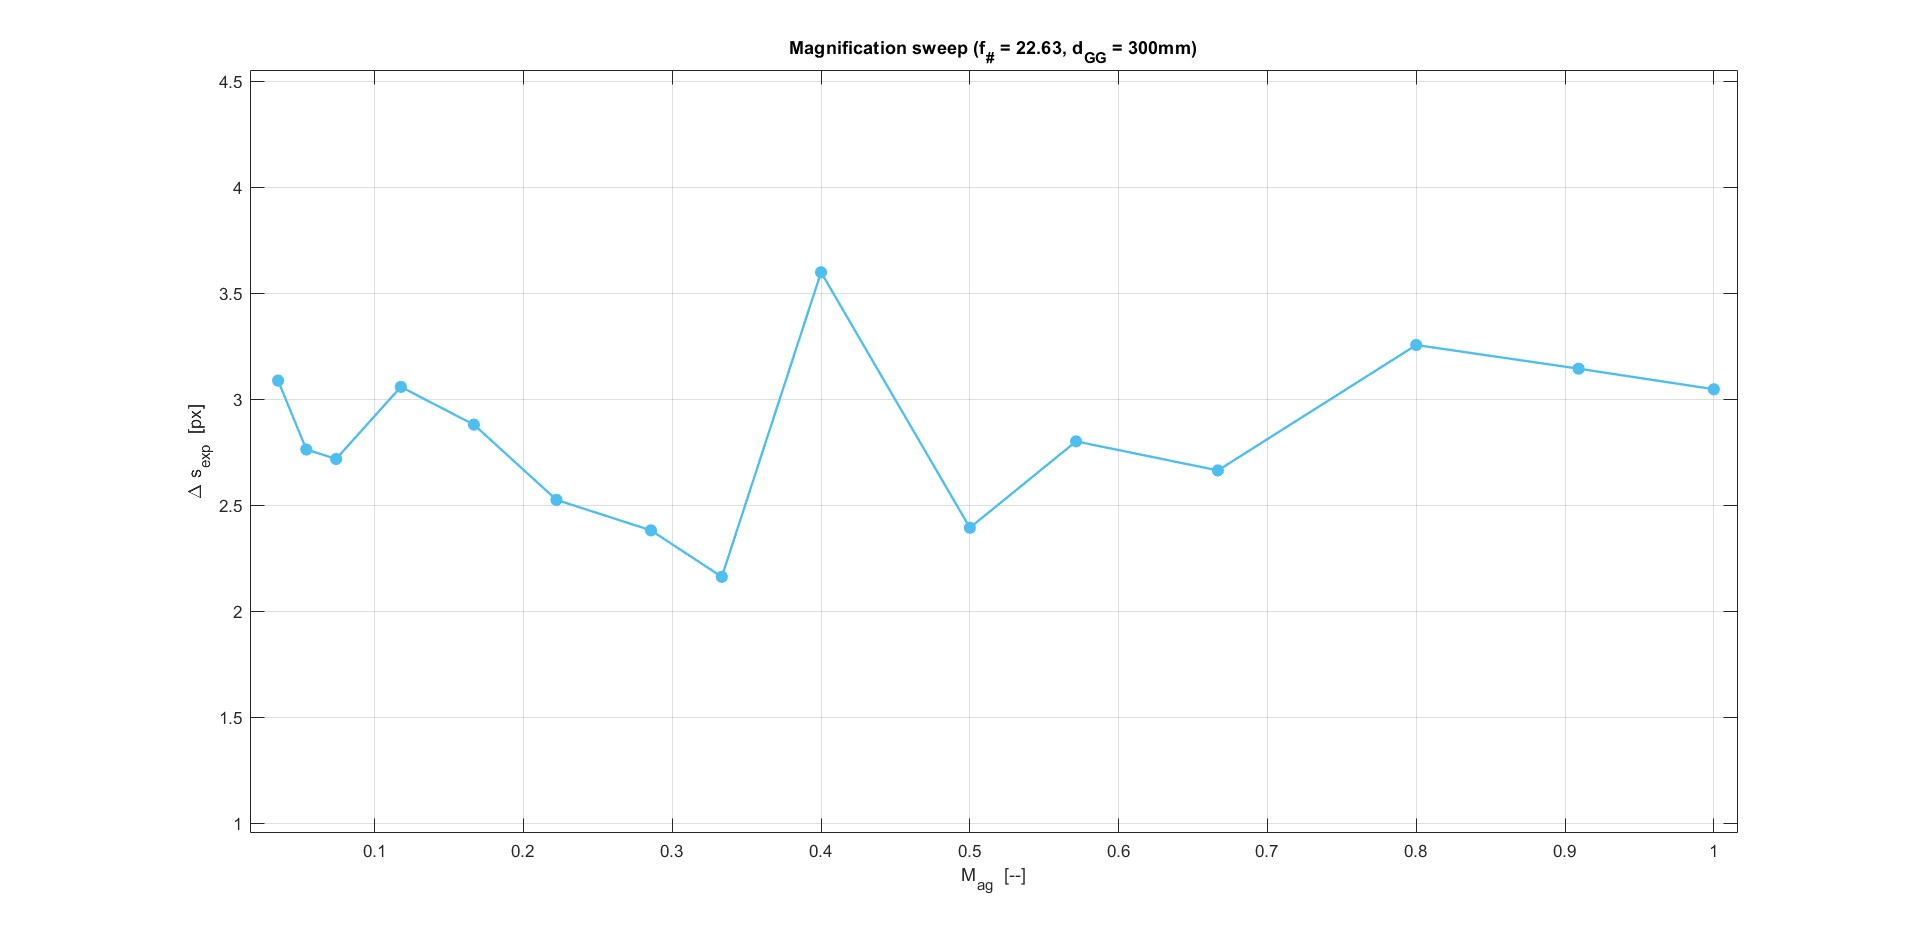
\includegraphics[width=\textwidth]{figures/speckle exp mag sweep.jpg}
    \caption{Average speckle size versus optical magnification for points 14--28 of Table \ref{tab: speckle results}, acquired at a fixed $f_\# = 22.63$ and $d_{GG} = 300$ mm. The magnification of these points was obtained from the distance marks of the camera lens rather than with the calibration plate}
    \label{fig: speckle magnification sweep}
\end{figure}

The speckle pattern investigation campaign allowed for the study of the speckle generation process. It successfully reproduced finer speckles than the angled glass experiment, showed the dependence of the speckle size on the f-stop number, investigated the effect of a small incidence beam in the diffuser and compared direct with projected speckle. However, the data showed unexpected insensitivity to magnification variations and still deviated significantly from the speckle predicted through the Rayleigh limit. It is worth reiterating that the speckle generation process is a complex intrinsically random phenomenon and to treat it with much more detail would be out of the scope of this thesis. For now, the data at hand make it possible to define a laser speckle generator capable of producing speckles within the 2--5 pixel range. Therefore, the findings of this campaign are enough to proceed to the correct application of Laser Speckled BOS to image a real schlieren object, in this case a compressible jet.


\section{Compressible Jet Experiment Results}
\label{section: Compressible Jet Experiment Results}

% REVIEW: NPR_g in the subfigure captions of the next figure is not defined anywhere. This introduction also promises a quantitative density field, but that subsection is still empty.
An underexpanded compressible jet was chosen as the object of study for the implementation of SBOS to a real schlieren object. The goal of this experiment was to image the jet at various nozzle pressure ratios ($NPR$), post-process the raw displacement data into a quantitative density field, analyze the jet structure and study the influence of an increase in nozzle pressure. The setup of this experiment was explained in Section \ref{section: Compressible jet experiment}. Figure \ref{fig: compressible jet displacement fields} displays the results of the cross correlation for the 6 different gauge pressures set at the wall air tap.

\begin{figure}[htbp]
    \centering
    \begin{subfigure}[b]{0.32\textwidth}
        \centering
        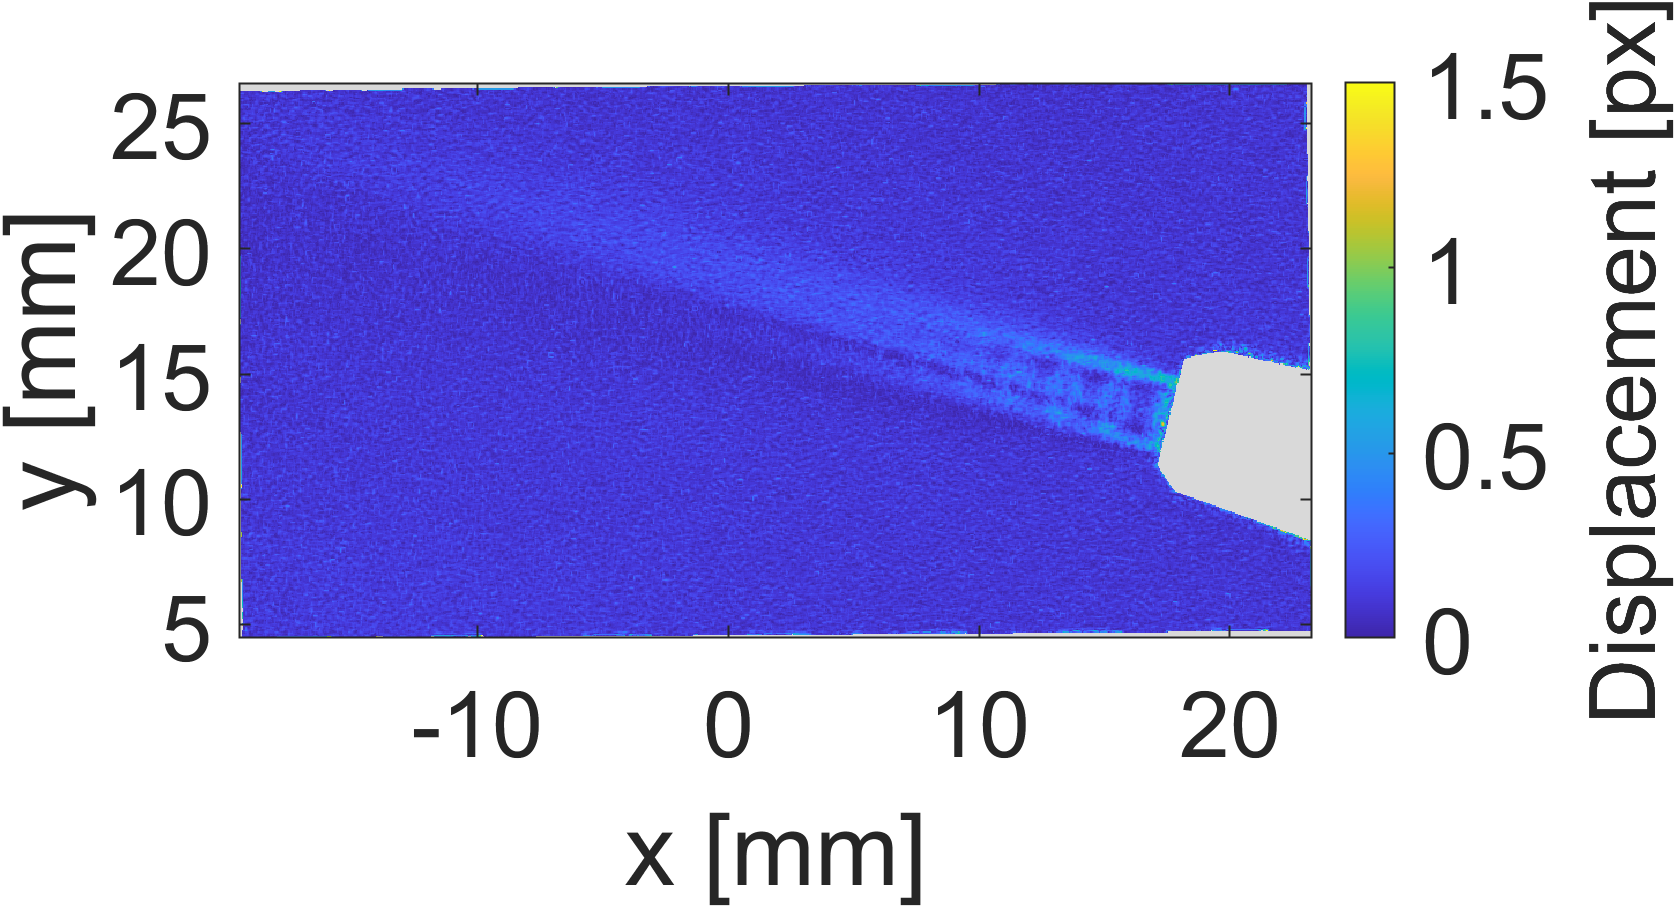
\includegraphics[width=\textwidth]{figures/jet displacement 3bar.png}
        \caption{$p_g = 3$ bar, with respective $NPR_g = 3.96$}
        \label{fig: jet displacement 3bar}
    \end{subfigure}
    \hfill
    \begin{subfigure}[b]{0.32\textwidth}
        \centering
        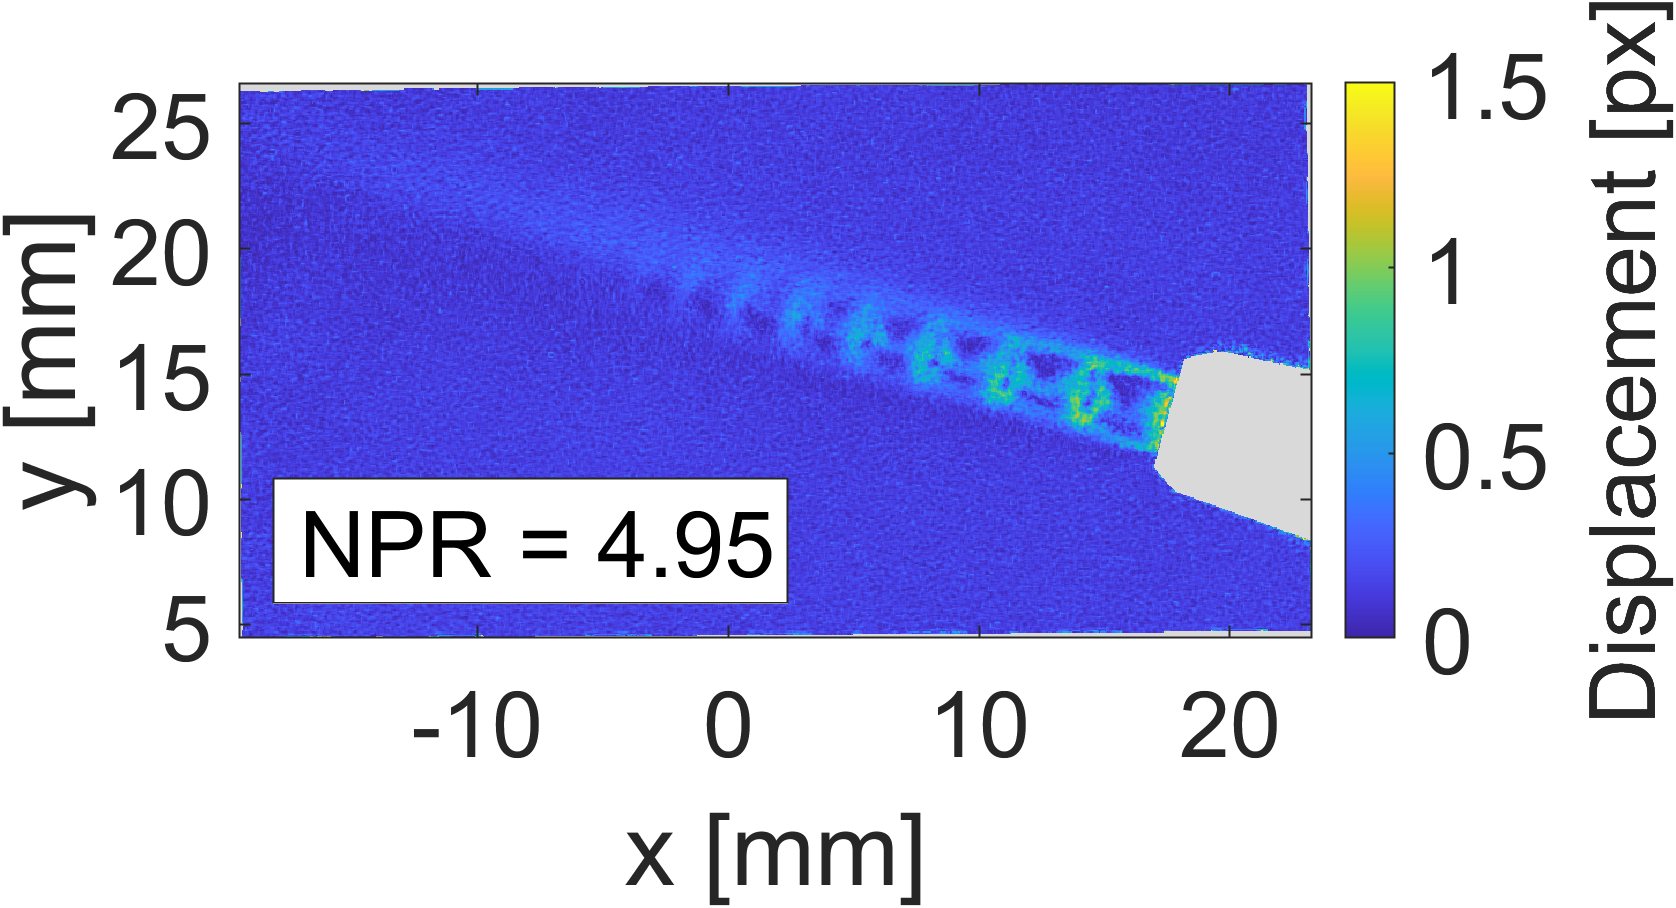
\includegraphics[width=\textwidth]{figures/jet displacement 4bar.png}
        \caption{$p_g = 4$ bar, with respective $NPR_g = 4.95$}
        \label{fig: jet displacement 4bar}
    \end{subfigure}
    \hfill
    \begin{subfigure}[b]{0.32\textwidth}
        \centering
        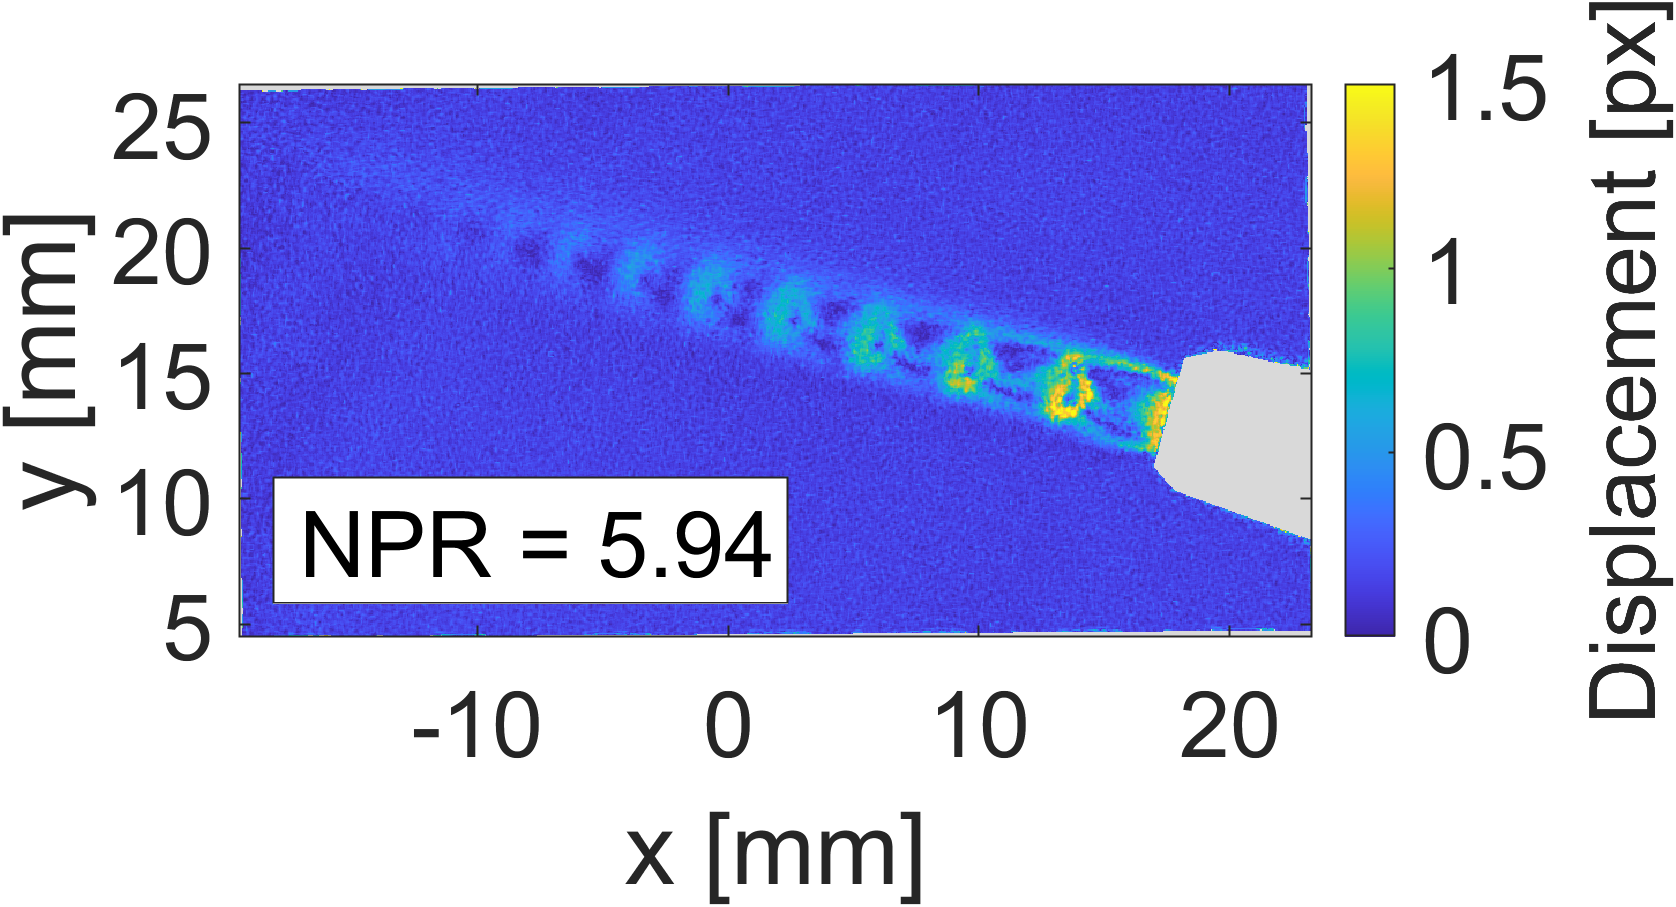
\includegraphics[width=\textwidth]{figures/jet displacement 5bar.png}
        \caption{$p_g = 5$ bar, with respective $NPR_g = 5.94$}
        \label{fig: jet displacement 5bar}
    \end{subfigure}

    \vspace{0.5em}

    \begin{subfigure}[b]{0.32\textwidth}
        \centering
        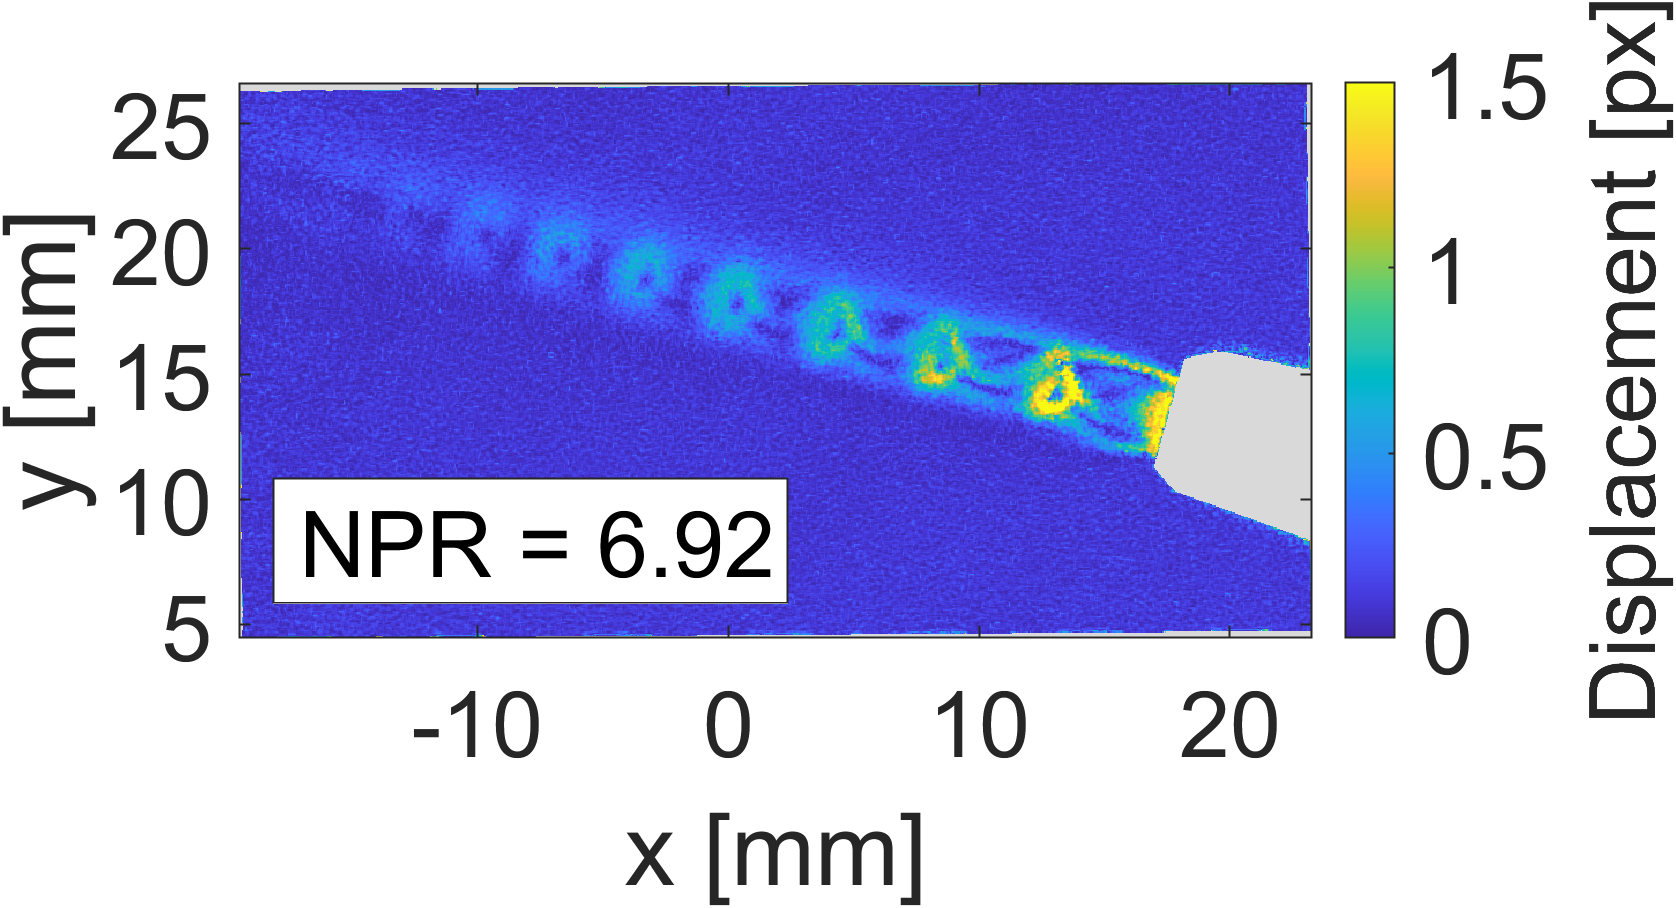
\includegraphics[width=\textwidth]{figures/jet displacement 6bar.png}
        \caption{$p_g = 6$ bar, with respective $NPR_g = 6.92$}
        \label{fig: jet displacement 6bar}
    \end{subfigure}
    \hfill
    \begin{subfigure}[b]{0.32\textwidth}
        \centering
        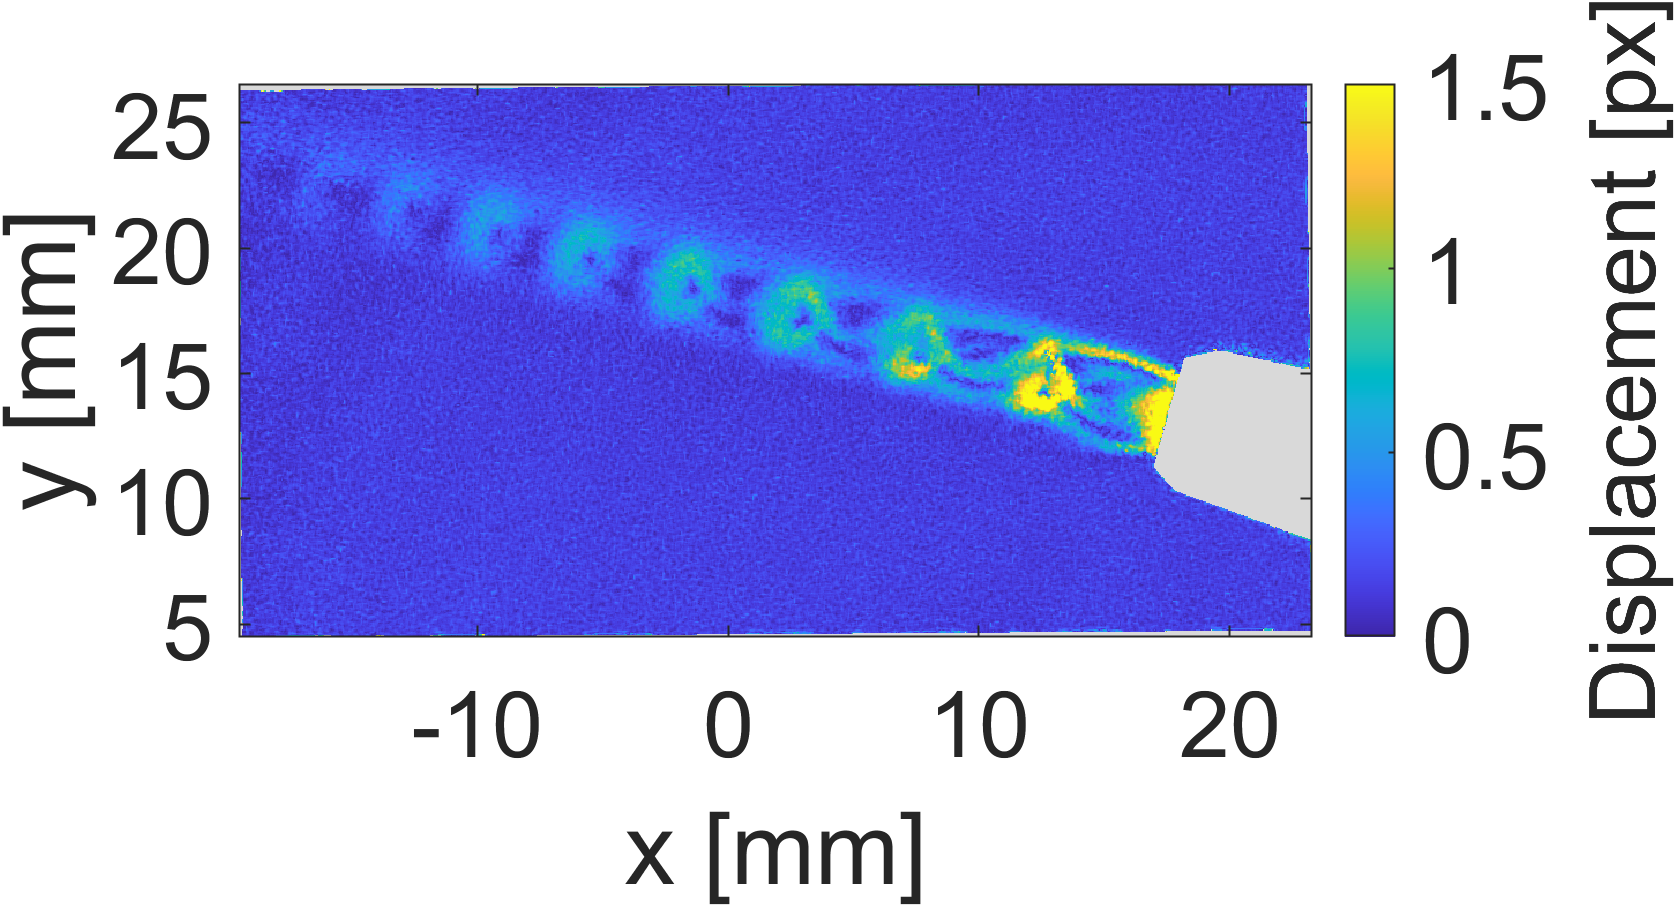
\includegraphics[width=\textwidth]{figures/jet displacement 7bar.png}
        \caption{$p_g = 7$ bar, with respective $NPR_g = 7.91$}
        \label{fig: jet displacement 7bar}
    \end{subfigure}
    \hfill
    \begin{subfigure}[b]{0.32\textwidth}
        \centering
        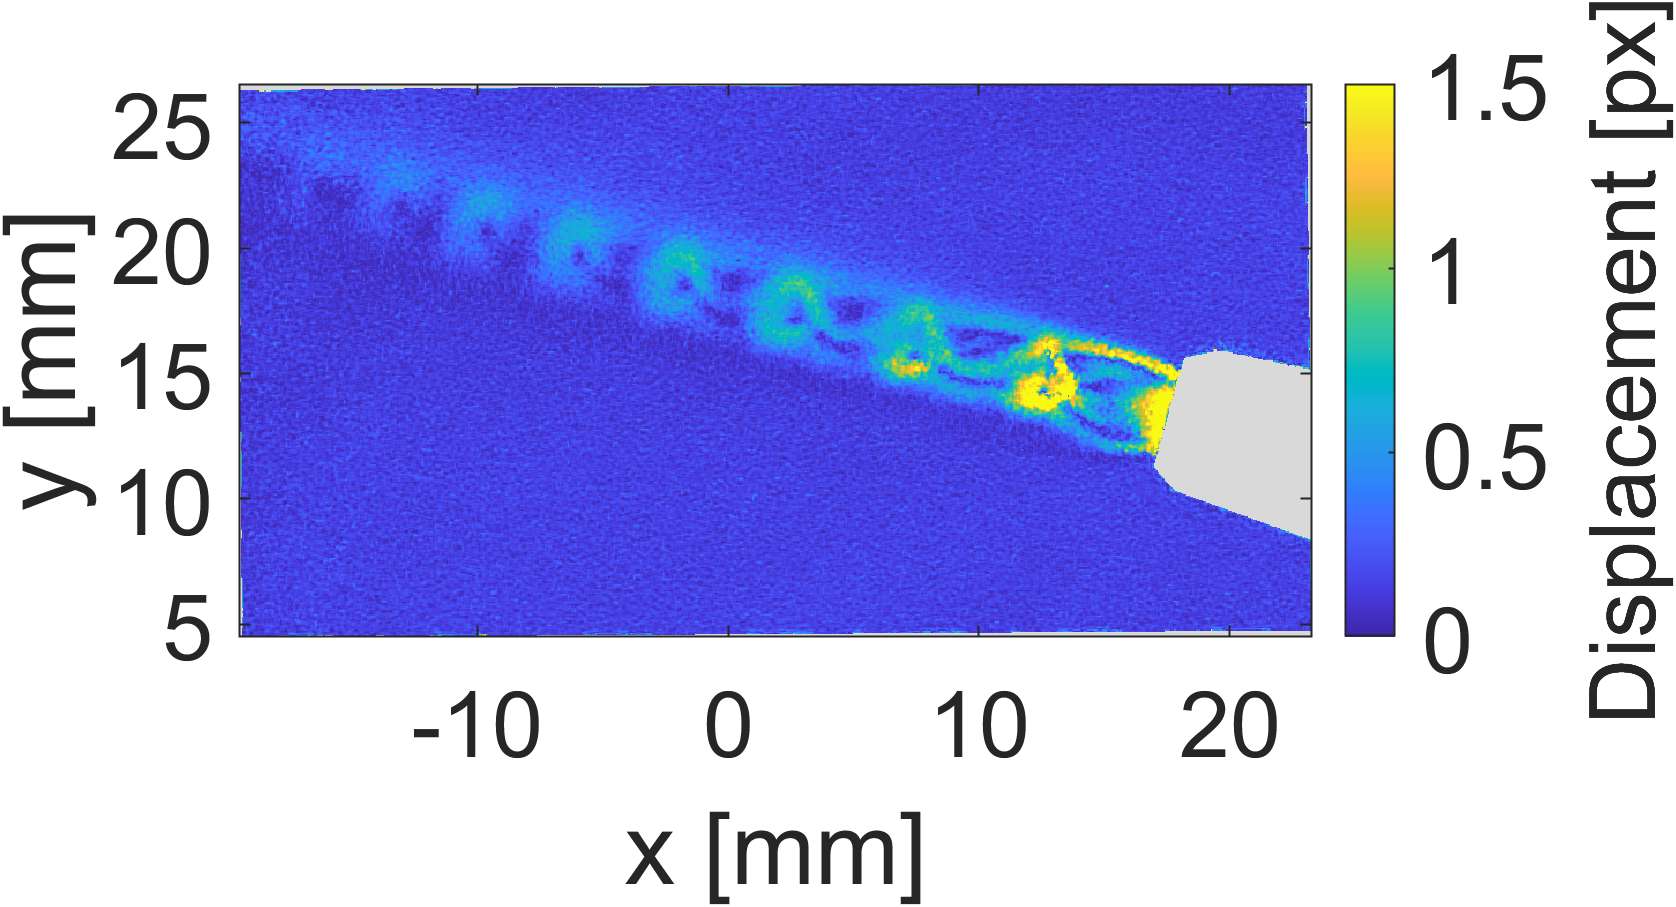
\includegraphics[width=\textwidth]{figures/jet displacement 8bar.png}
        \caption{$p_g = 8$ bar, with respective $NPR_g = 8.90$}
        \label{fig: jet displacement 8bar}
    \end{subfigure}
    \caption{SBOS results for a compressible jet. Displacement magnitude fields obtained through cross correlation for air tap gauge pressures from 3 bar to 8 bar with a step of 1 bar. All fields share the same color scale and masked vectors are shown in grey}
    \label{fig: compressible jet displacement fields}
\end{figure}

% REVIEW: the 7 and 8 bar cases have NPR_g = 7.91 and 8.90, above the 4 to 7 range, so they would fall in the single barrel regime.
Comparing the different images displayed by Figure \ref{fig: compressible jet displacement fields}, it is possible to assess the effect of different $NPR$ to the underexpanded jet structure. As explained in Section \ref{section: Compressible Jet Theory}, an increase in $NPR$ leads to an increase in shock cell length and a fundamental change in the jet structure at certain pressure ranges. Comparing the result for $p_g = 3$ bar to $p_g = 8$ bar, the shock cell length does indeed increase, together with the number of cells and a bigger bulge mid-cell. However, there is very little change in the shock cell length for gauge pressures 6 through 8 bar. Moreover, from Figure \ref{fig: jet displacement 4bar} onward the $NPR$ is within 4 to 7 so the formation of a Mach disk together with a "barrel" shaped shock cell would be expected, see Figure \ref{fig: highly underexpanded jet}. Nevertheless, all images seem to display an "X" shape, related to a nozzle pressure ratio of 2 to 4, Figure \ref{fig: moderately underexpanded jet}. Together, these deviations from theory indicate that the real pressure ratios at the nozzle are not what they would be if the total pressure were maintained from the wall air tap gauge, through the hose and out of the air gun. Therefore, there must be heavy pressure losses present throughout the line that need to be accounted for and new estimates of the nozzle pressure ratios must be computed.

% REVIEW: the text says p_e is obtained, but Table 6.9 reports p_0. The uncertainties are said to correspond to +1 deg in nu, but rows b to e use the -1 deg bound and row a the smaller bound. Row a rests on nu = 1 deg with a 1 deg reading uncertainty; consider commenting on that precision.
The strategy envisioned to better estimate the nozzle pressure ratio builds on top of the definition of the Prandtl-Meyer angle. As explained in Section \ref{section: Compressibility}, $\nu$ is the turning angle needed for a flow at a certain Mach number $M_1$ to expand to a Mach number $M_2$. In the case studied, the flow is choked at the nozzle exit, so the Mach number at the exit is assumed to be equal to one $M_e = 1$. At the lip, the flow expands isentropically until it reaches a certain $M_j$ at ambient pressure. Therefore, the angle of the flow at the shear layer is equal to $\varphi = \nu(M_j)$ relative to the jet axis. So, to better estimate the $NPR$, the images were then treated to make the jet axis horizontal, then the shear layer angle at the lip was measured, $M_j$ was calculated through the Prandtl-Meyer function and a value for $p_e$ was obtained using isentropic expansion. The values can be found in Table \ref{tab: compressible jet NPR estimates} together with the uncertainty corresponding to $+ 1^\circ$ in $\nu$.

\begin{table}[htbp]
    \centering
    \caption{Estimated jet conditions for each Prandtl-Meyer angle $\nu$. $M_j$ is the jet Mach number, $NPR$ the nozzle pressure ratio and $p_0$ the absolute total pressure. The uncertainties $u_{M_j}$, $u_{NPR}$ and $u_{p_0}$ are given relative to their respective values. The data is organized in letters from "a)" to "f)", corresponding to the order of the images in Figure \ref{fig: compressible jet displacement fields}}
    \label{tab: compressible jet NPR estimates}
    \begin{tabular}{lrrrrrrr}
        \toprule
        Data & $\nu$ & $M_j$ & $u_{M_j}$ & $NPR$ & $u_{NPR}$ & $p_0$ & $u_{p_0}$ \\
             & [$^{\circ}$] & [-] & [\%] & [-] & [\%] & [bar] & [\%] \\
        \midrule
        a) &  1 & 1.082 & 4.71 & 2.088 & 6.51 & 2.115 & 6.52 \\
        b) &  3 & 1.177 & 3.74 & 2.353 & 5.48 & 2.384 & 5.49 \\
        c) &  5 & 1.257 & 3.10 & 2.613 & 5.17 & 2.647 & 5.14 \\
        d) &  8 & 1.366 & 2.64 & 3.032 & 5.01 & 3.072 & 5.01 \\
        e) & 10 & 1.435 & 2.44 & 3.344 & 5.02 & 3.387 & 5.02 \\
        f) & 13 & 1.537 & 2.21 & 3.875 & 5.08 & 3.925 & 5.10 \\
        \bottomrule
    \end{tabular}
\end{table}

% REVIEW: e to f is the largest NPR step in Table 6.9 (3.344 to 3.875), not a small one. L_s changes least there (4.95 to 5.00 mm), which is also where the Emden fit diverges.
The $NPR$ estimates displayed in Table \ref{tab: compressible jet NPR estimates} better fit the theory but also mean that the pressure losses in the line were extremely high. The nozzle pressure ratios range from 2 to 4, exactly the range where an "X" shaped shock cell would be expected. Moreover, the pressures of datasets e and f change very little between them, while there is a big difference between a and f, which is coherent with the similar pictures obtained. A question arises, however, when the estimate of total pressure is compared with the one at the air tap gauge, as loss of over 40\% cannot be explained with friction losses alone. These other sources of loss were probably choke points in the line, at quick disconnect joints or at a non-fully pressed air gun trigger. Another way to verify these estimates is by computing the density gradient field, measuring the shock cell length and relating them to the NPR through the relationships of Section \ref{section: Compressible Jet Theory}, this way validating it with literature data.

A density gradient field can be obtained assuming a planar field, through Equation \ref{equation: Displacement and Density Gradient}. This result corresponds to the projection of the axisymmetric body. In reality, the thickness of the object $W$ and the density gradient vary with the radius, so this solution will underestimate the density gradients at the borders of the jet. Nevertheless, it is useful to qualitatively study the shock cell structure, as the periodicity of the cell and the gradient signs are maintained in the projection. Figure \ref{fig: dataset f density gradients} shows the gradients for dataset f in the two directions s and n together with the magnitude of the vector. For this application, the background of the image was removed by calculating the median vector of a window only containing the background, then the image was rotated and translated such that the jet axis is horizontal and corresponds to n = 0.

\begin{figure}[htbp]
    \centering
    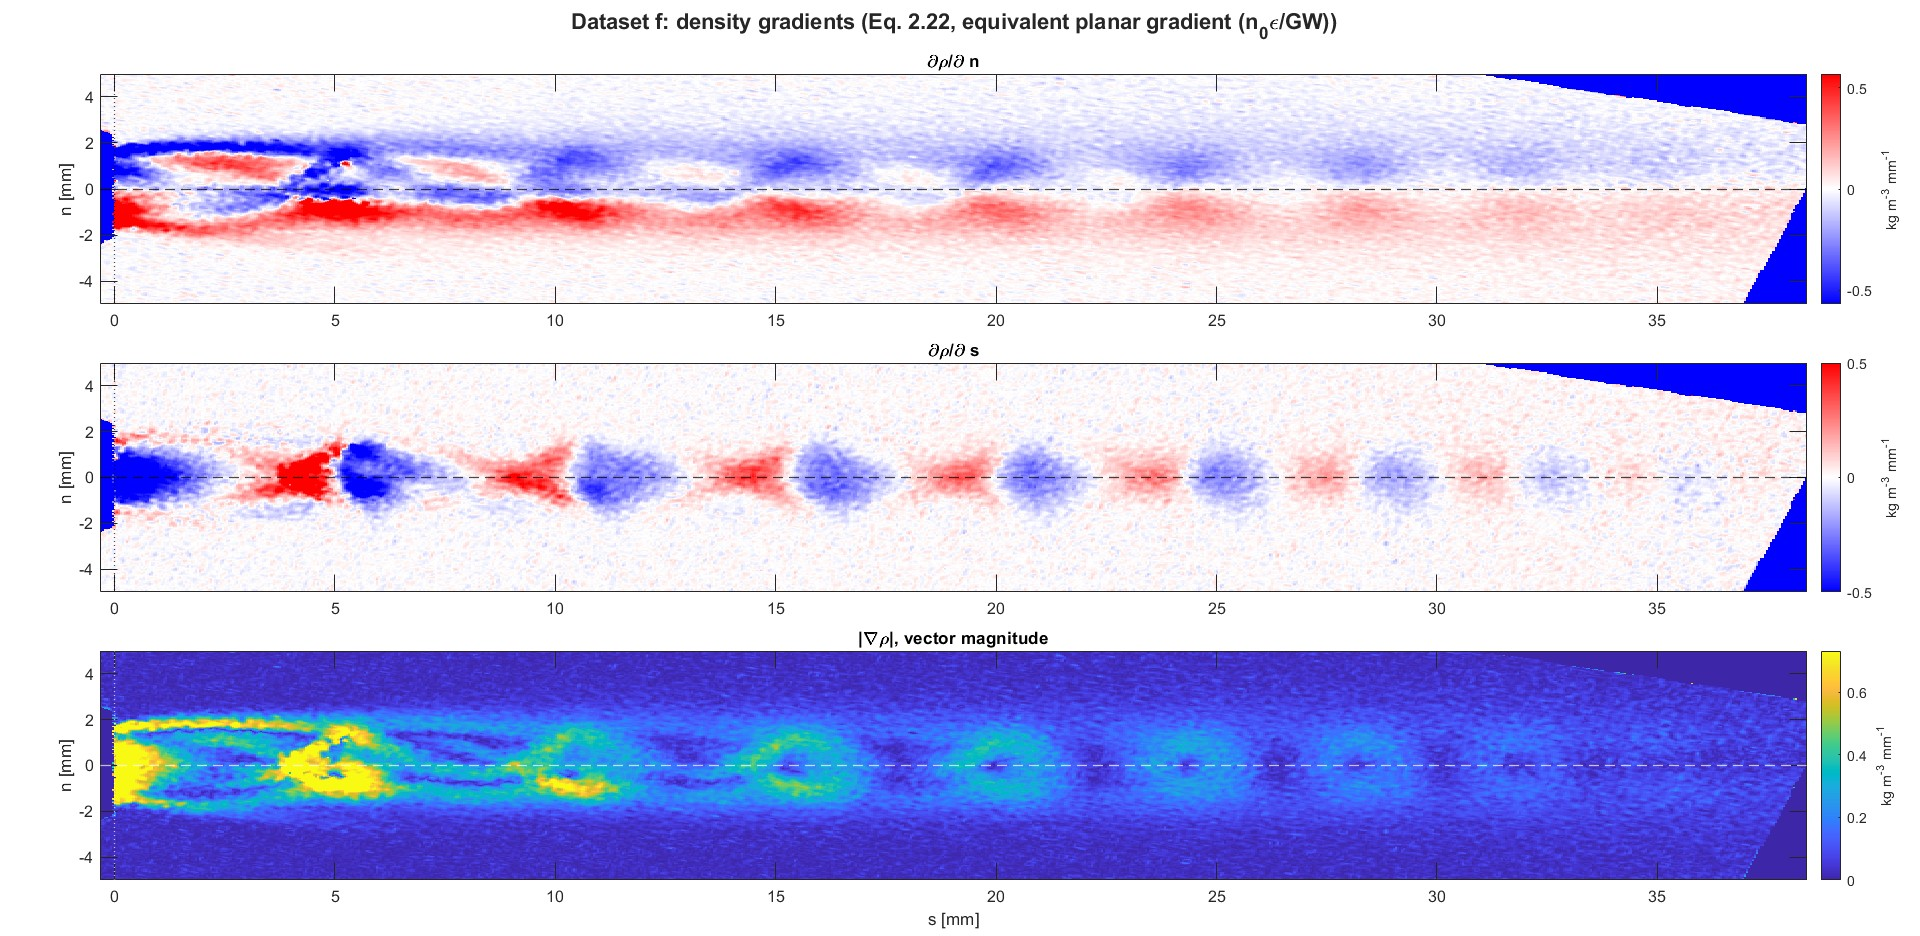
\includegraphics[width=\textwidth]{figures/Dataset f density gradients.jpg}
    \caption{Density gradient fields of dataset f obtained assuming a planar field. The top plot displays the density gradient in the n direction, the middle plot the density gradient in the s direction and the bottom plot the magnitude of the density gradient vector. The s axis is aligned with the jet axis with its origin at the nozzle exit, while n is normal to it}
    \label{fig: dataset f density gradients}
\end{figure}

Following the middle plot of Figure \ref{fig: dataset f density gradients}, correspondent to the density gradient in the s direction, the jet structures can be easily identified. Spanning from the lip to the axis at the nozzle exit, an expansion fan causes the density to decrease severely, indicated by the blue region in the core of the jet. A little above the lip, an oblique shock is marked in red going from the lip to the axis downstream, where it reflects in direction to the shear layer, forming an "X" shape. This intercepting shock produces a region of increasing density, marked in red. After the density peaks, a new round of expansion waves causes the density to decrease, thus starting a new shock cell. The periodicity of the shock cells is also evident if the centerline density gradient is plotted. Figure \ref{fig: centerline density gradients} displays such a graph for the 6 datasets.

\begin{figure}[htbp]
    \centering
    \begin{subfigure}[b]{0.32\textwidth}
        \centering
        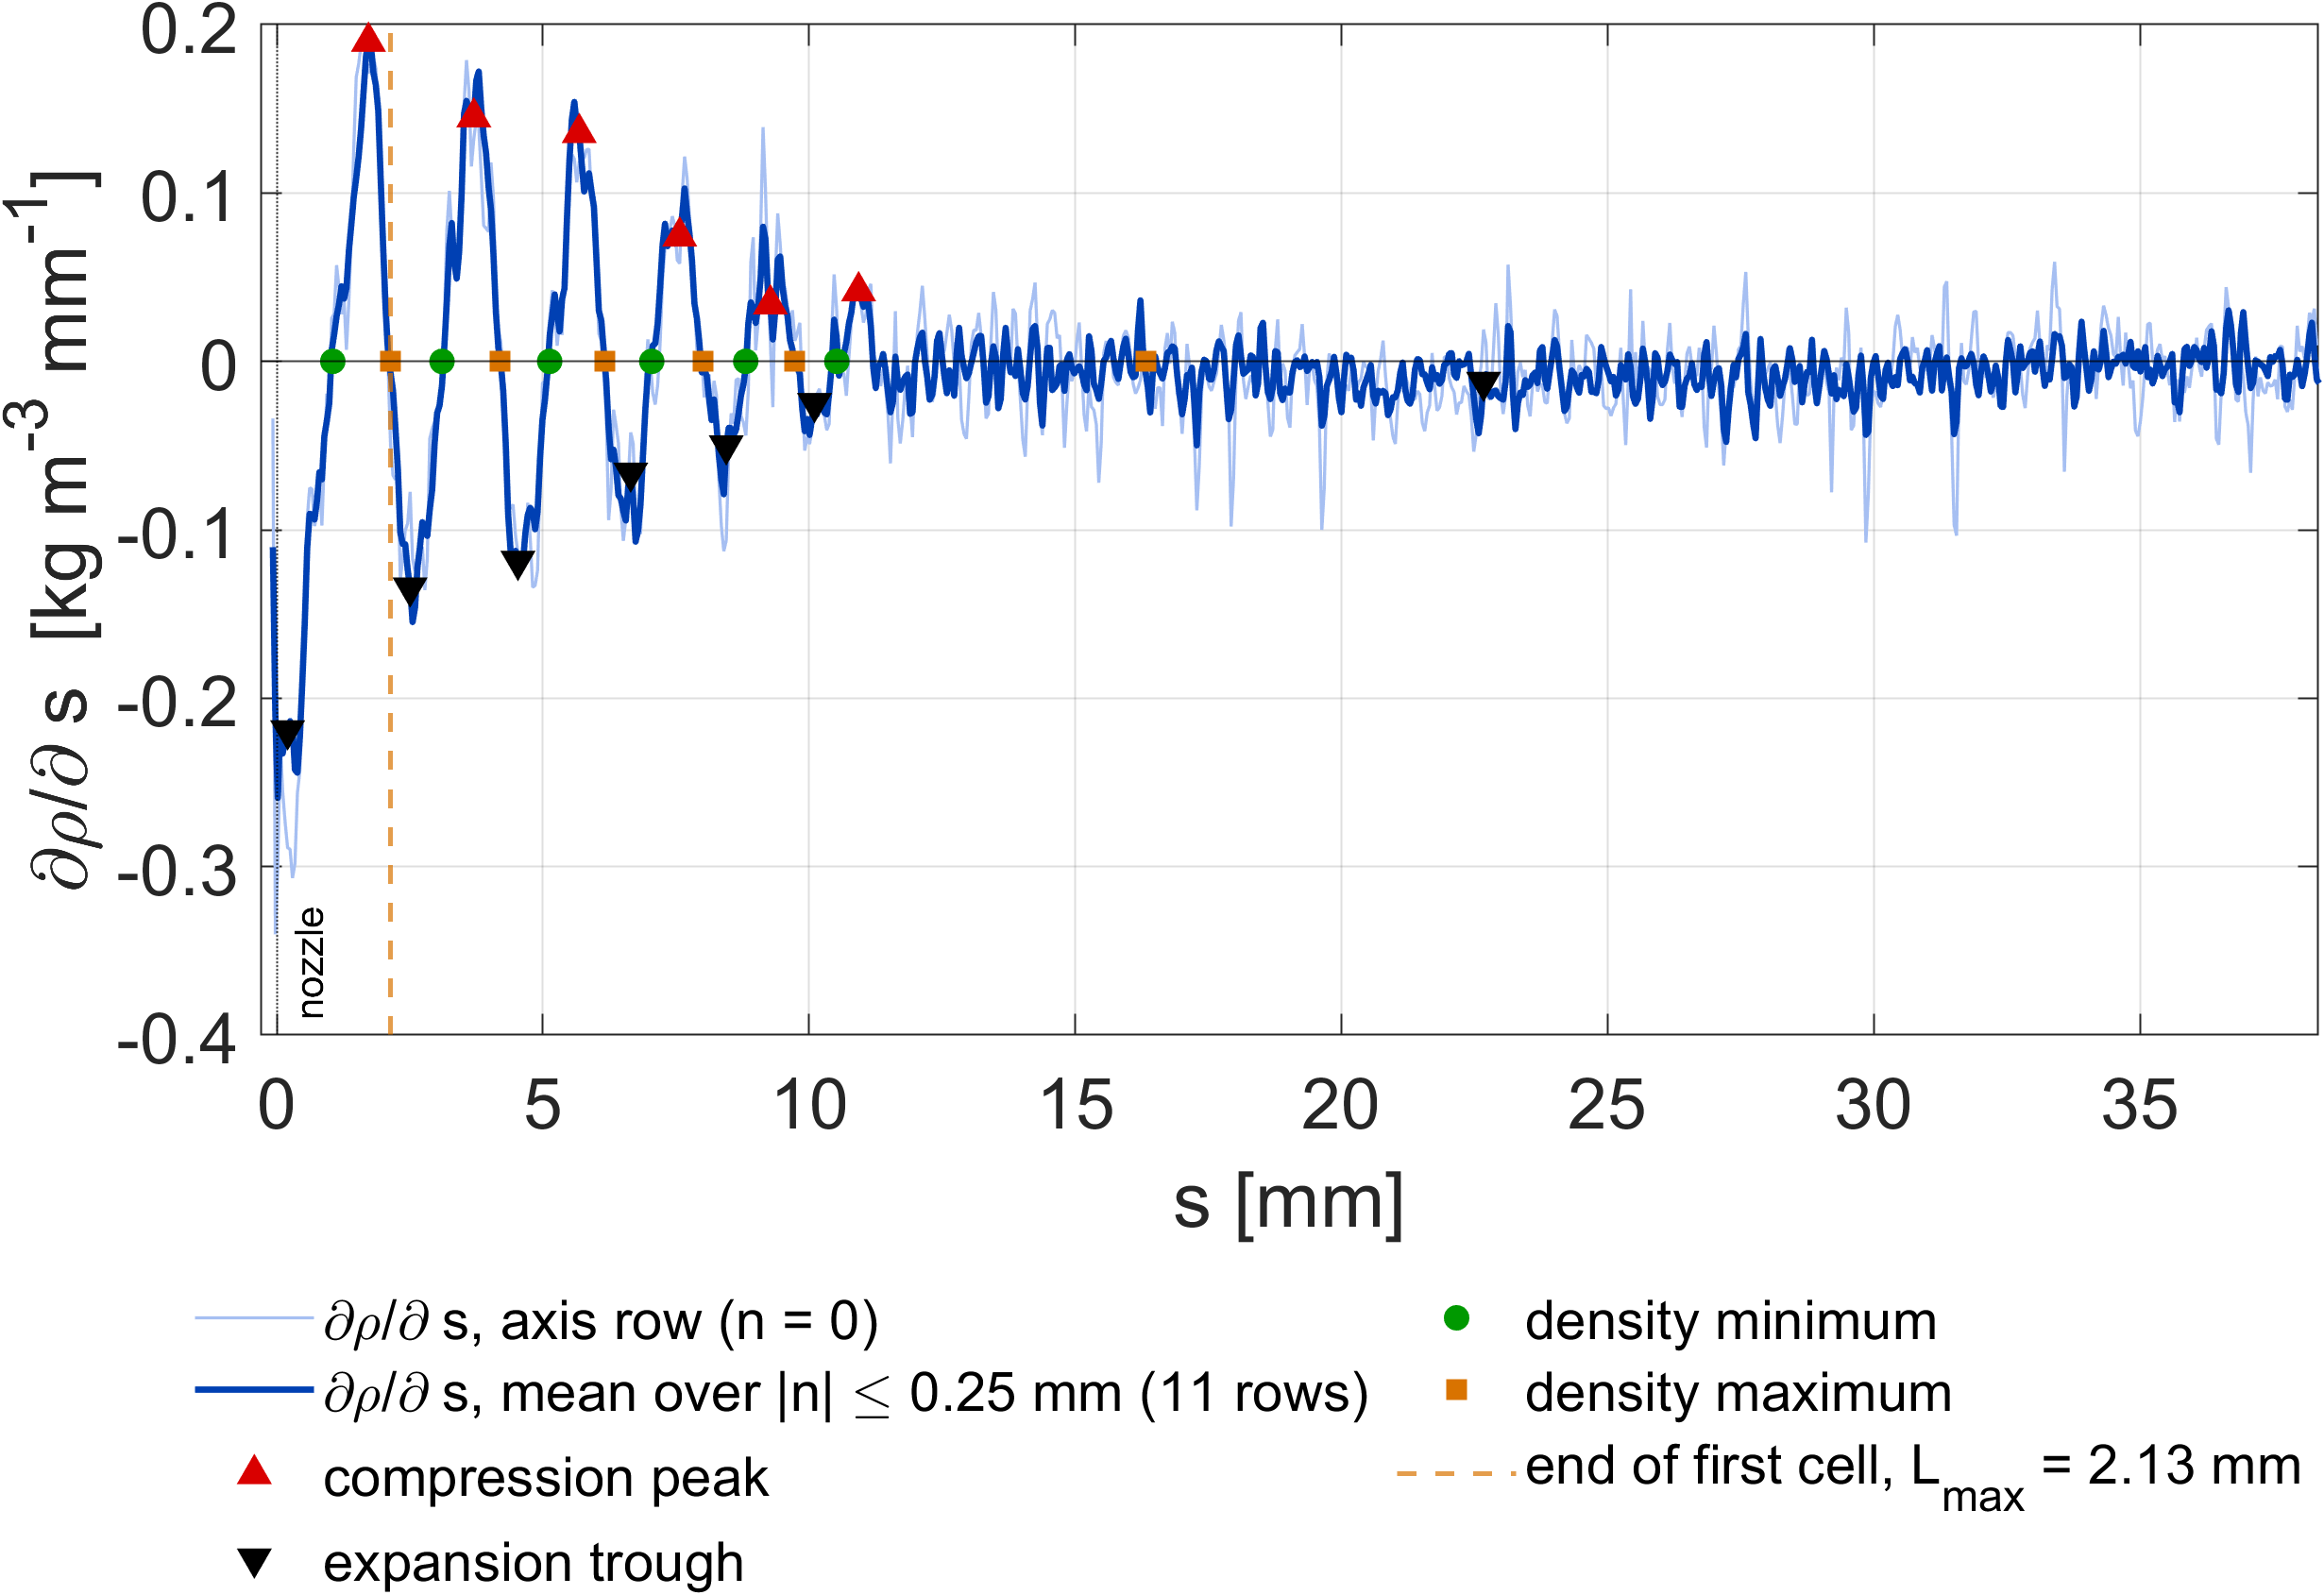
\includegraphics[width=\textwidth]{figures/centerline density gradient dataset a.png}
        \caption{Dataset a, with respective $NPR = 2.088$ and $L_s = 2.13$ mm}
        \label{fig: centerline density gradient dataset a}
    \end{subfigure}
    \hfill
    \begin{subfigure}[b]{0.32\textwidth}
        \centering
        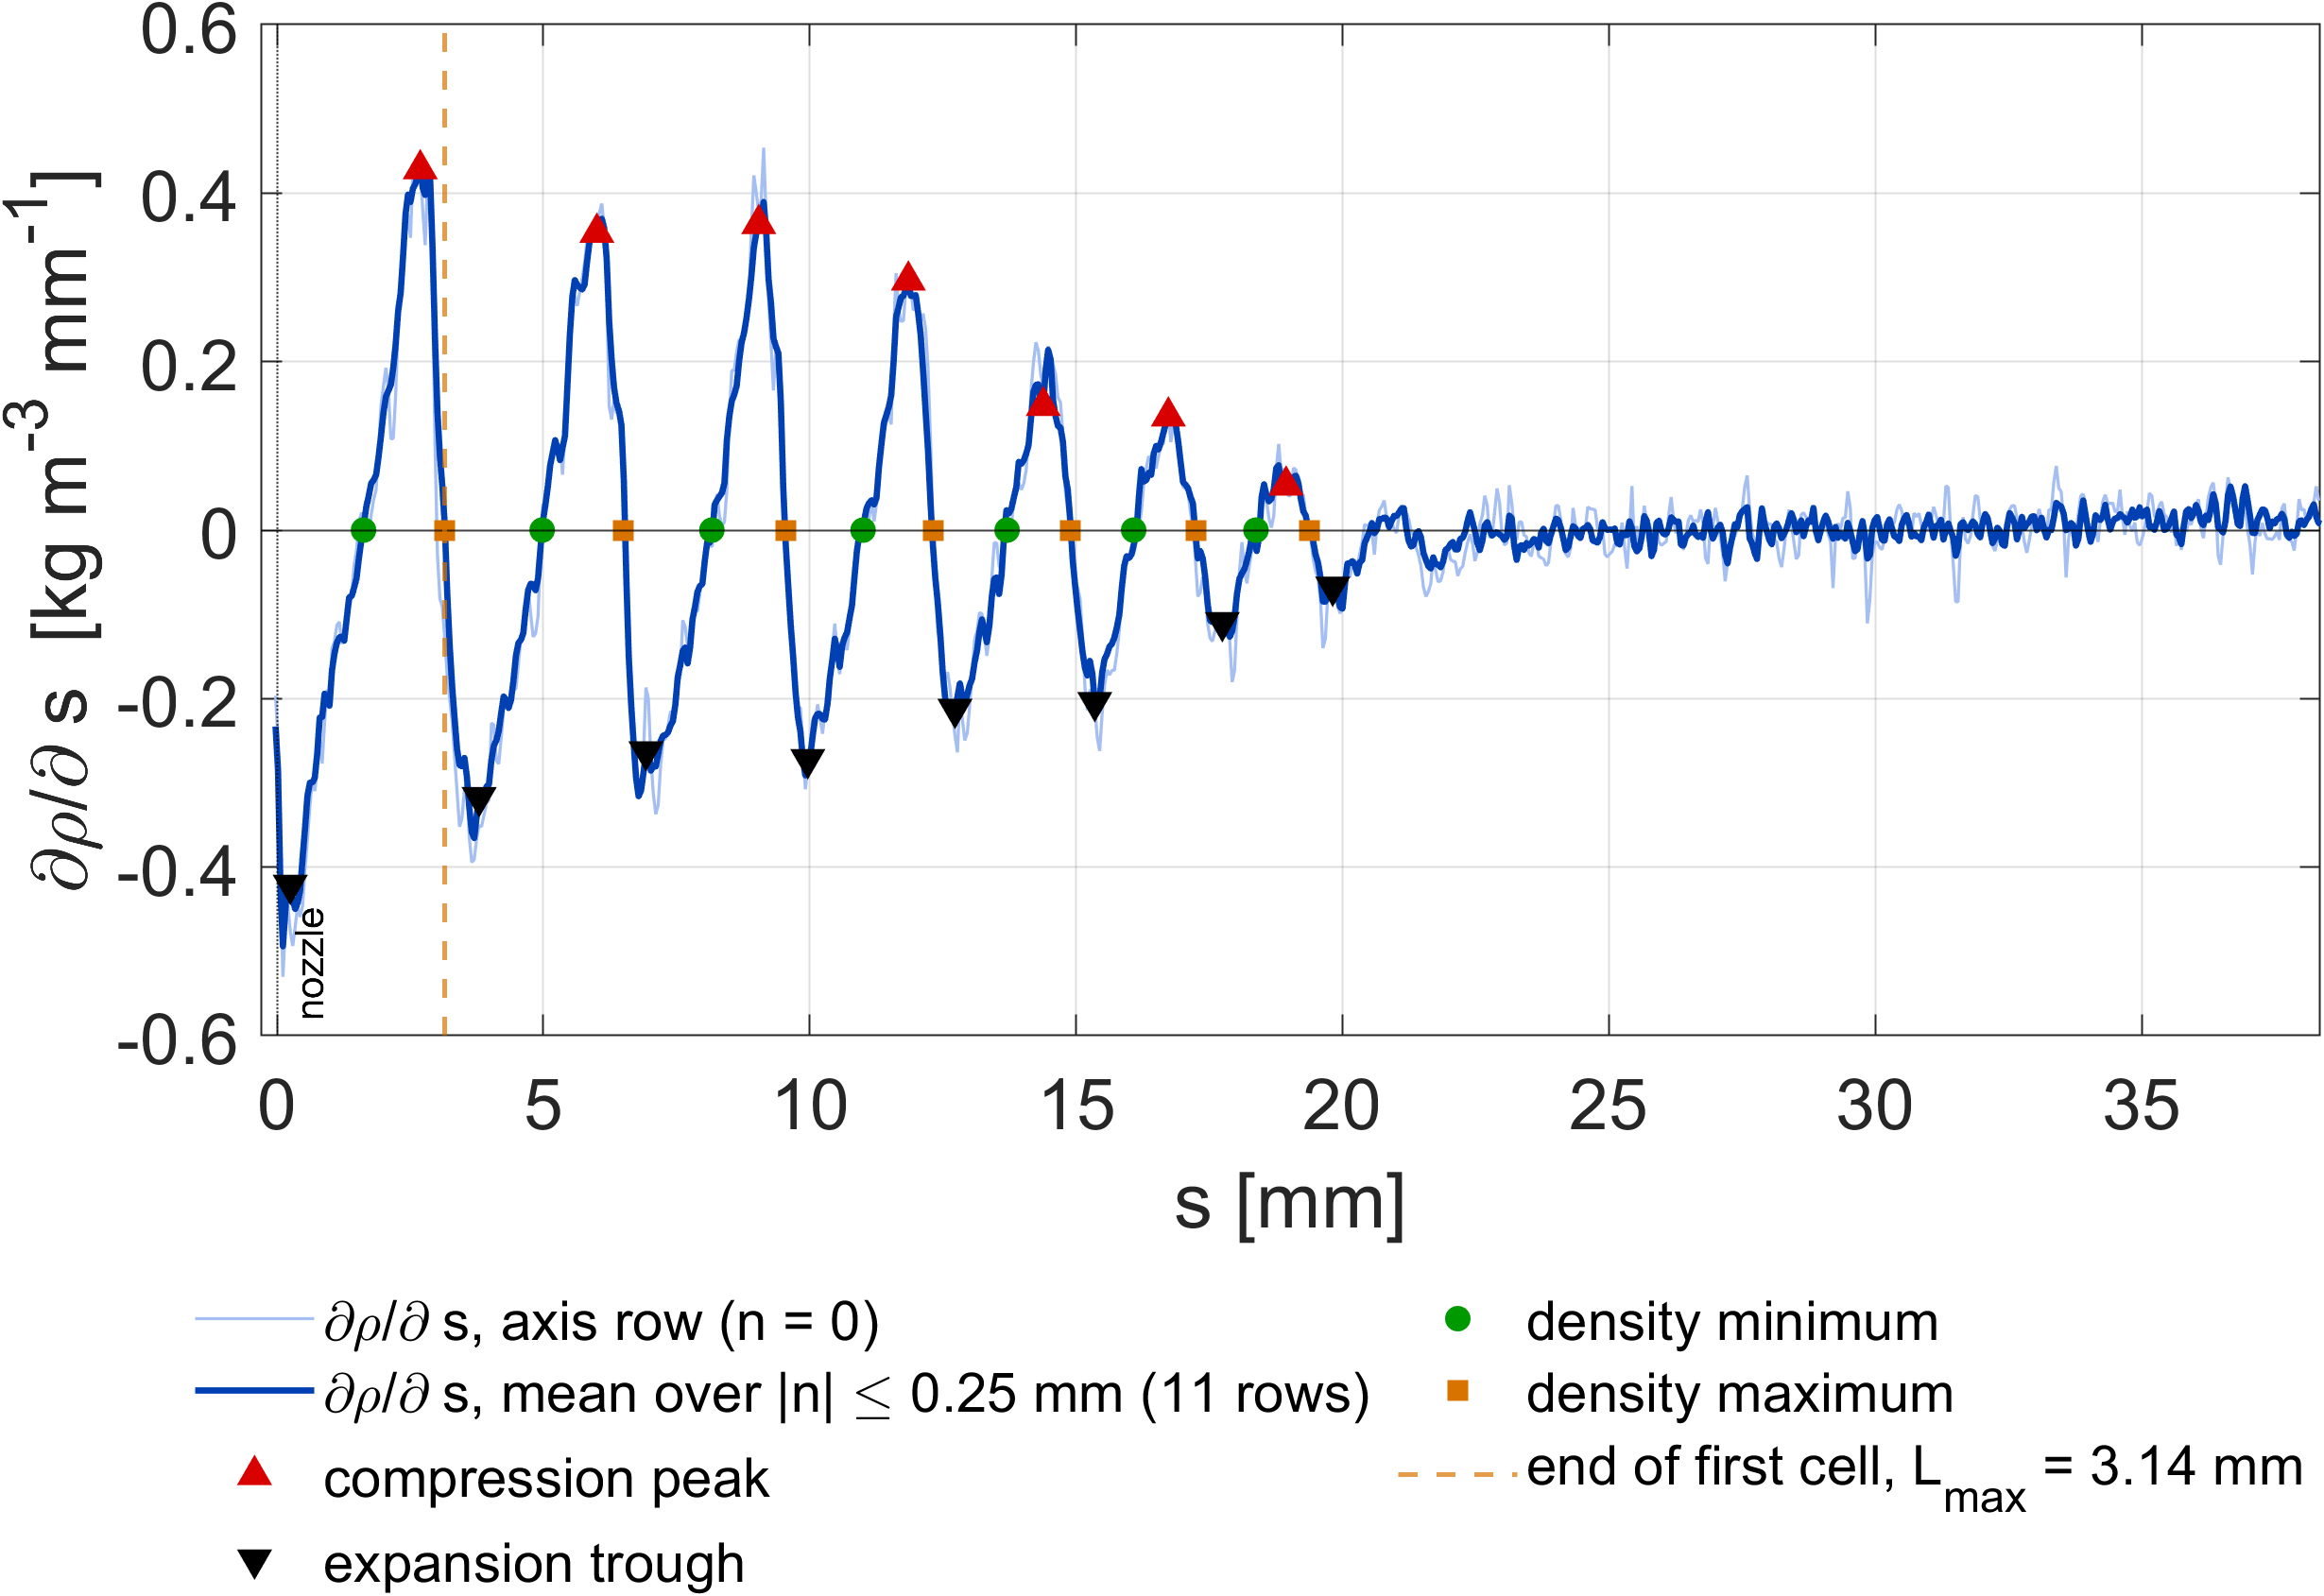
\includegraphics[width=\textwidth]{figures/centerline density gradient dataset b.png}
        \caption{Dataset b, with respective $NPR = 2.353$ and $L_s = 3.14$ mm}
        \label{fig: centerline density gradient dataset b}
    \end{subfigure}
    \hfill
    \begin{subfigure}[b]{0.32\textwidth}
        \centering
        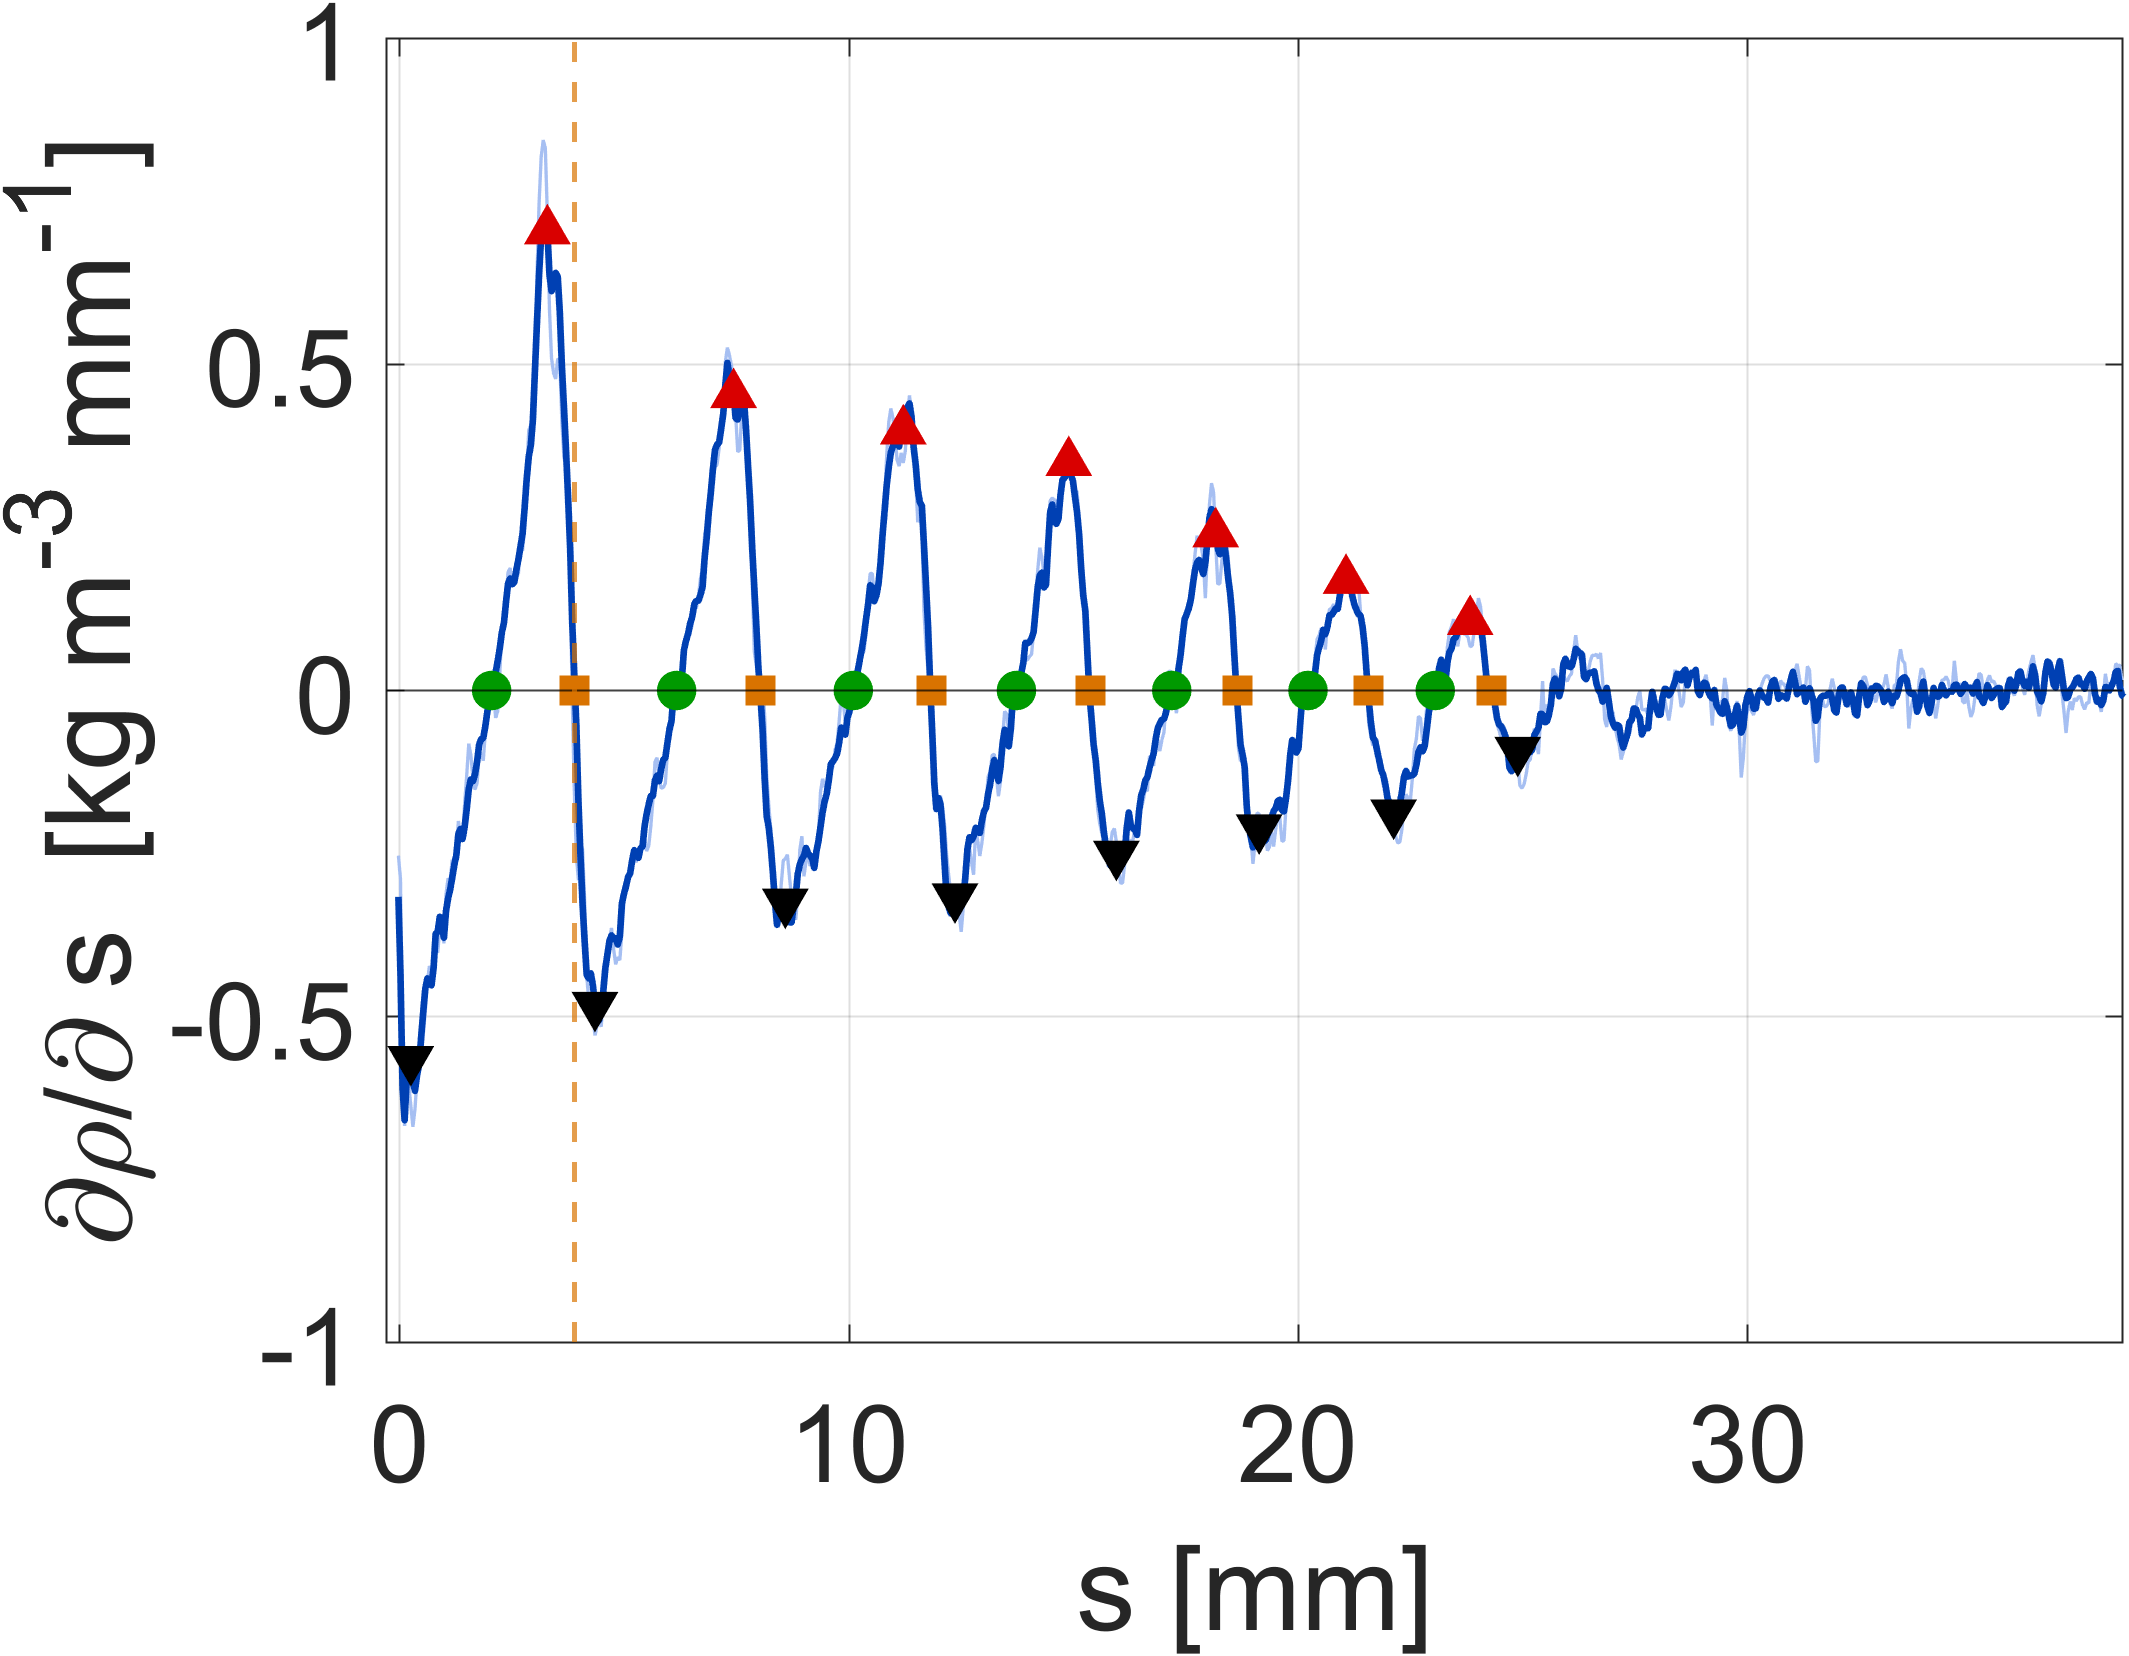
\includegraphics[width=\textwidth]{figures/centerline density gradient dataset c.png}
        \caption{Dataset c, with respective $NPR = 2.613$ and $L_s = 3.90$ mm}
        \label{fig: centerline density gradient dataset c}
    \end{subfigure}

    \vspace{0.5em}

    \begin{subfigure}[b]{0.32\textwidth}
        \centering
        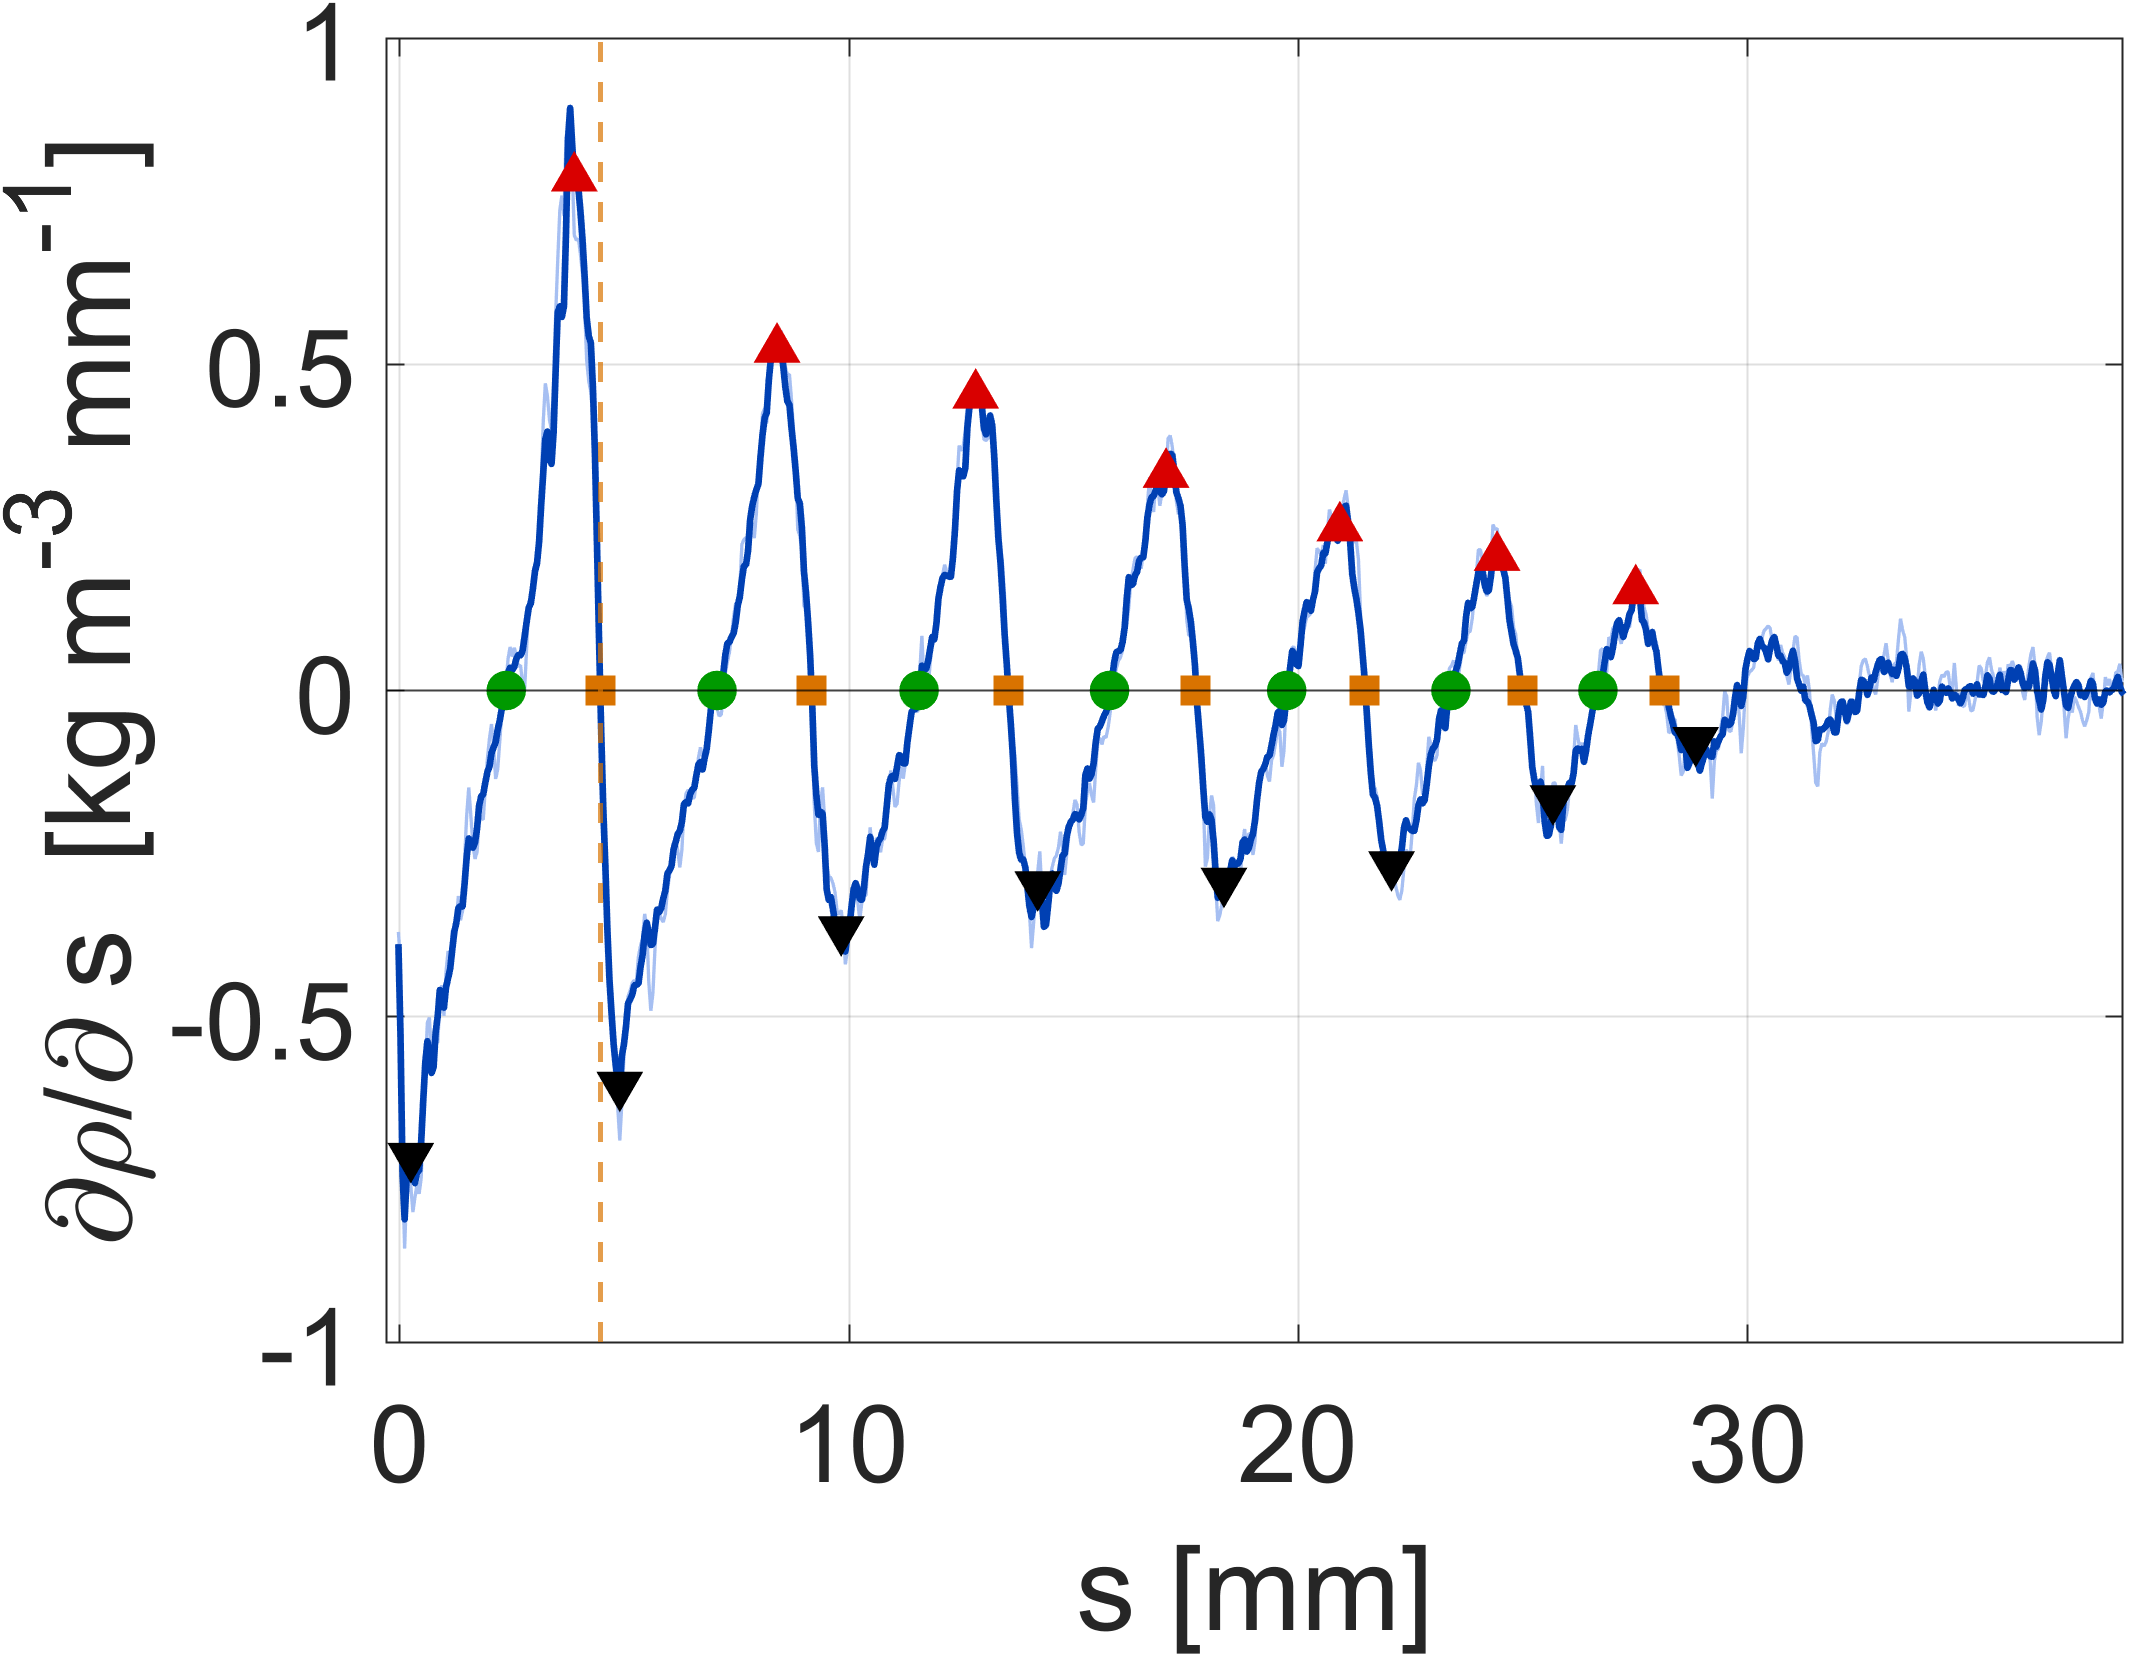
\includegraphics[width=\textwidth]{figures/centerline density gradient dataset d.png}
        \caption{Dataset d, with respective $NPR = 3.032$ and $L_s = 4.48$ mm}
        \label{fig: centerline density gradient dataset d}
    \end{subfigure}
    \hfill
    \begin{subfigure}[b]{0.32\textwidth}
        \centering
        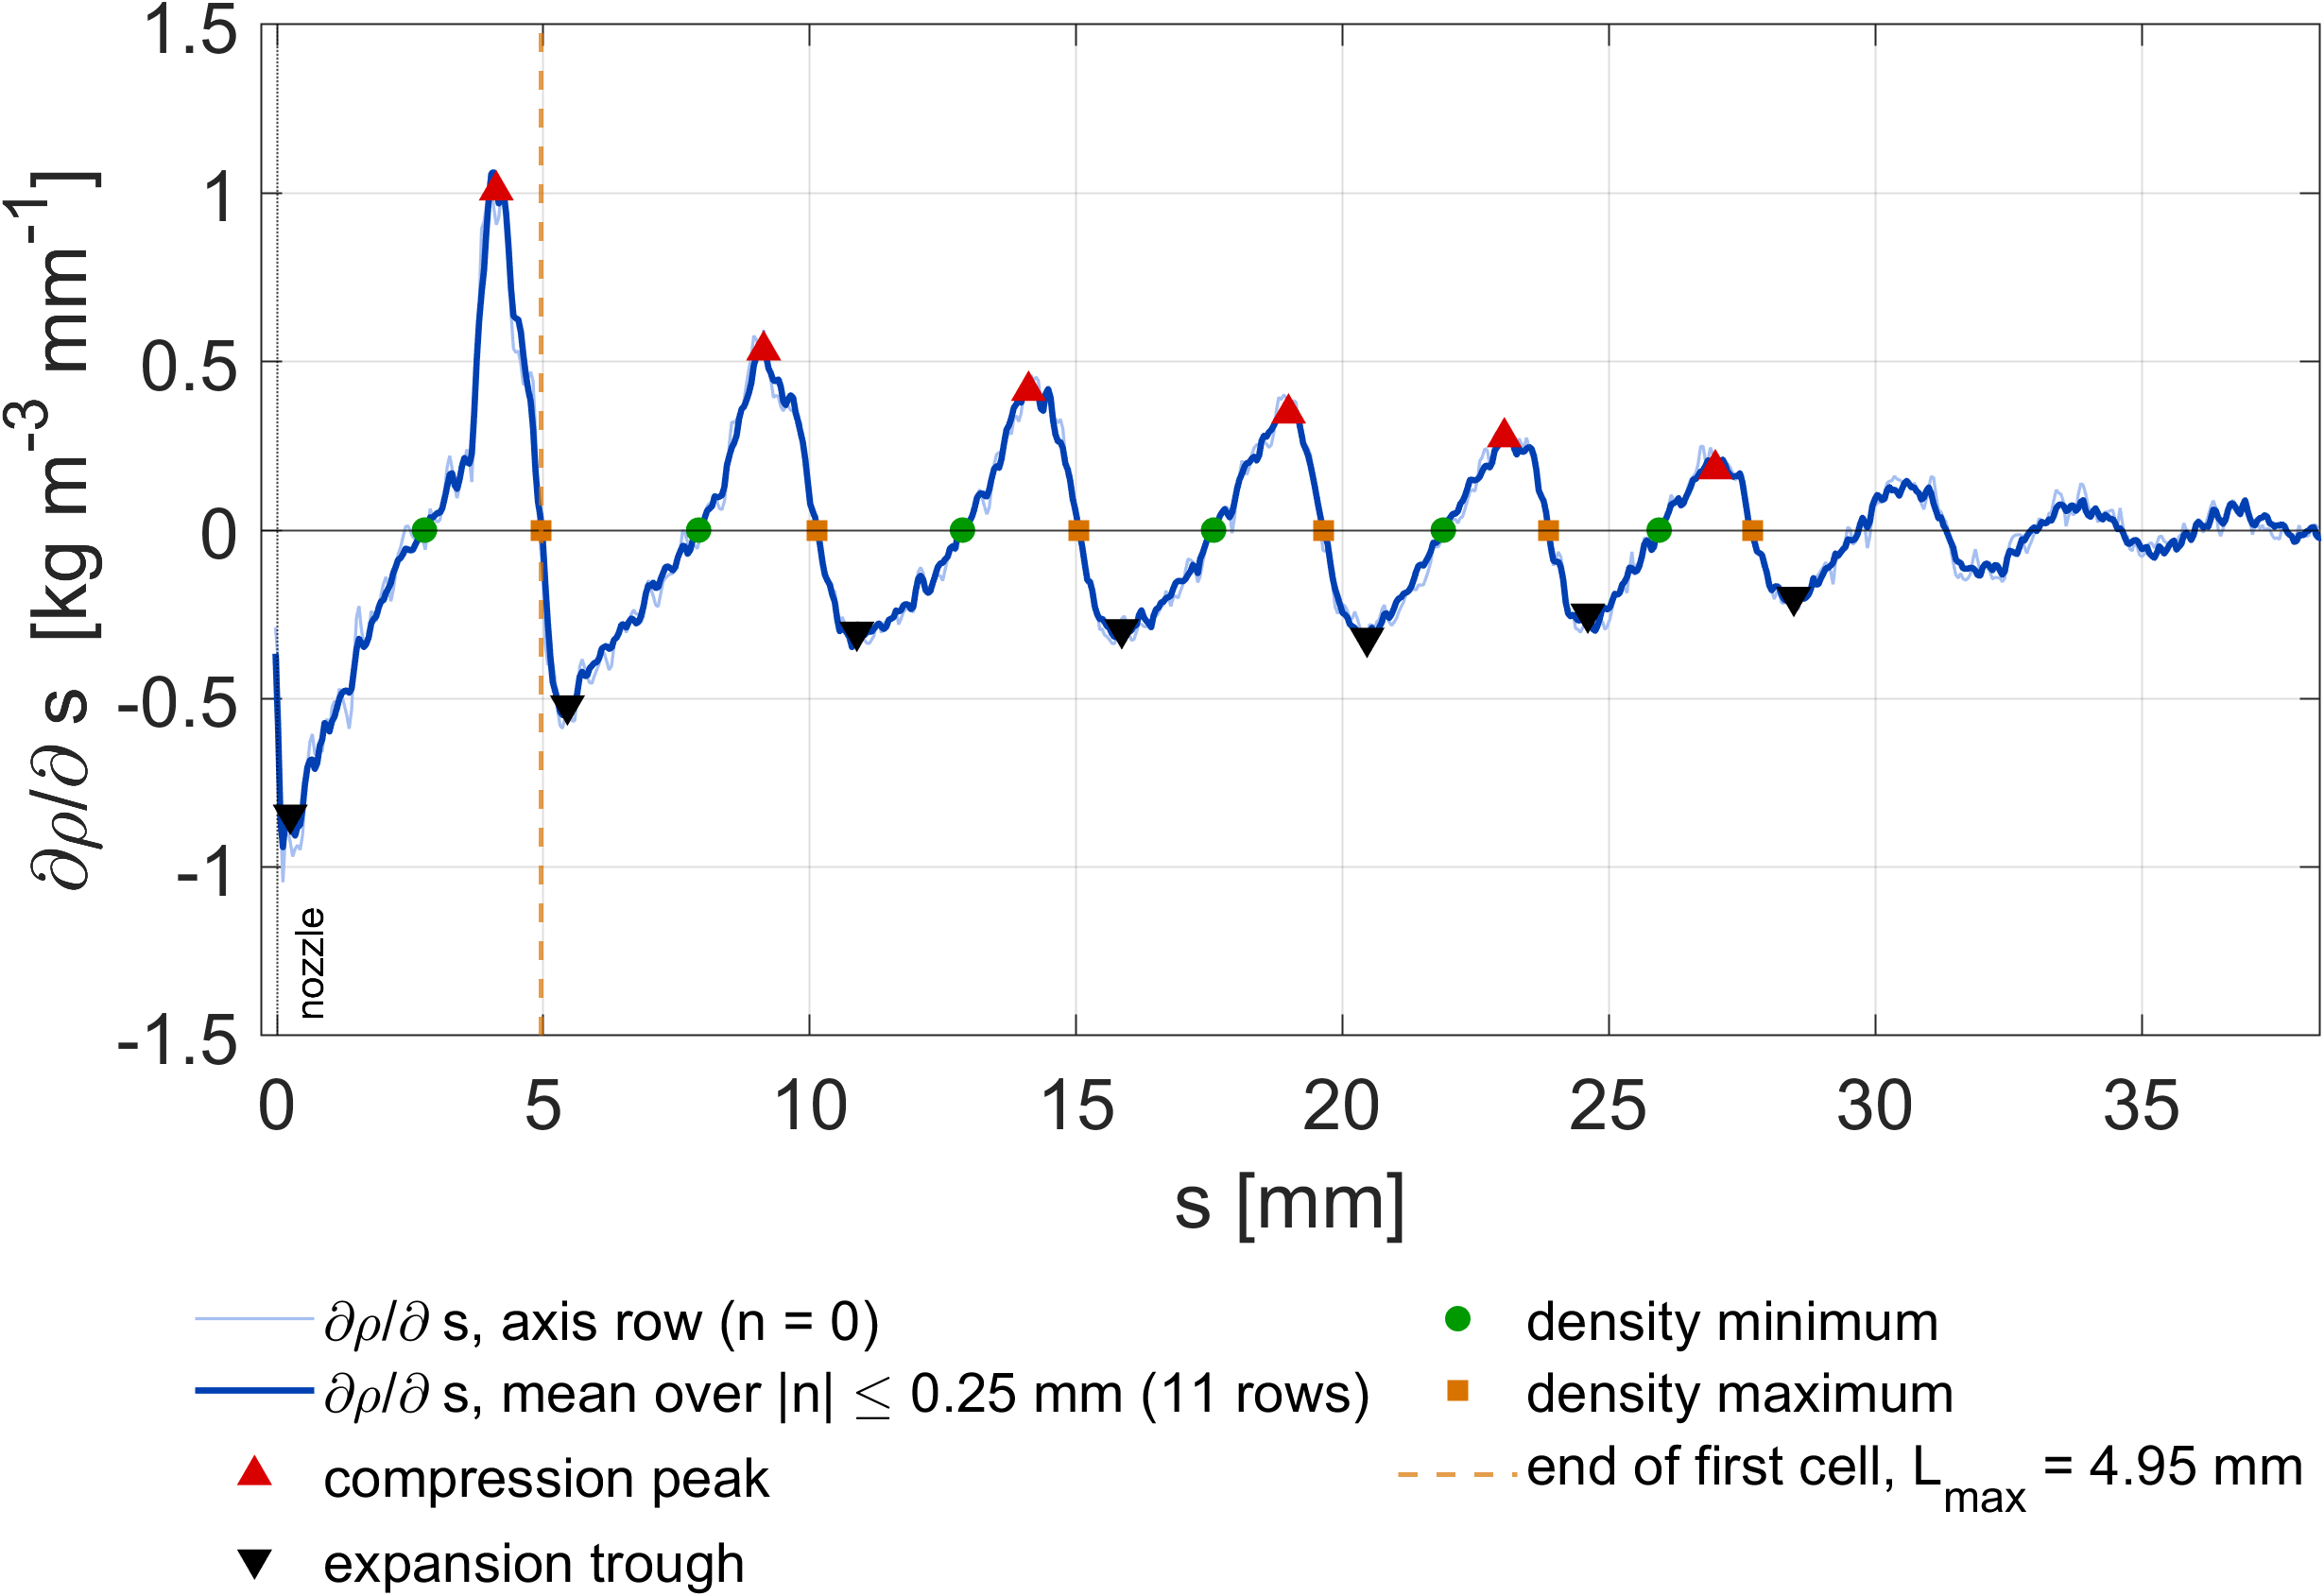
\includegraphics[width=\textwidth]{figures/centerline density gradient dataset e.png}
        \caption{Dataset e, with respective $NPR = 3.344$ and $L_s = 4.95$ mm}
        \label{fig: centerline density gradient dataset e}
    \end{subfigure}
    \hfill
    \begin{subfigure}[b]{0.32\textwidth}
        \centering
        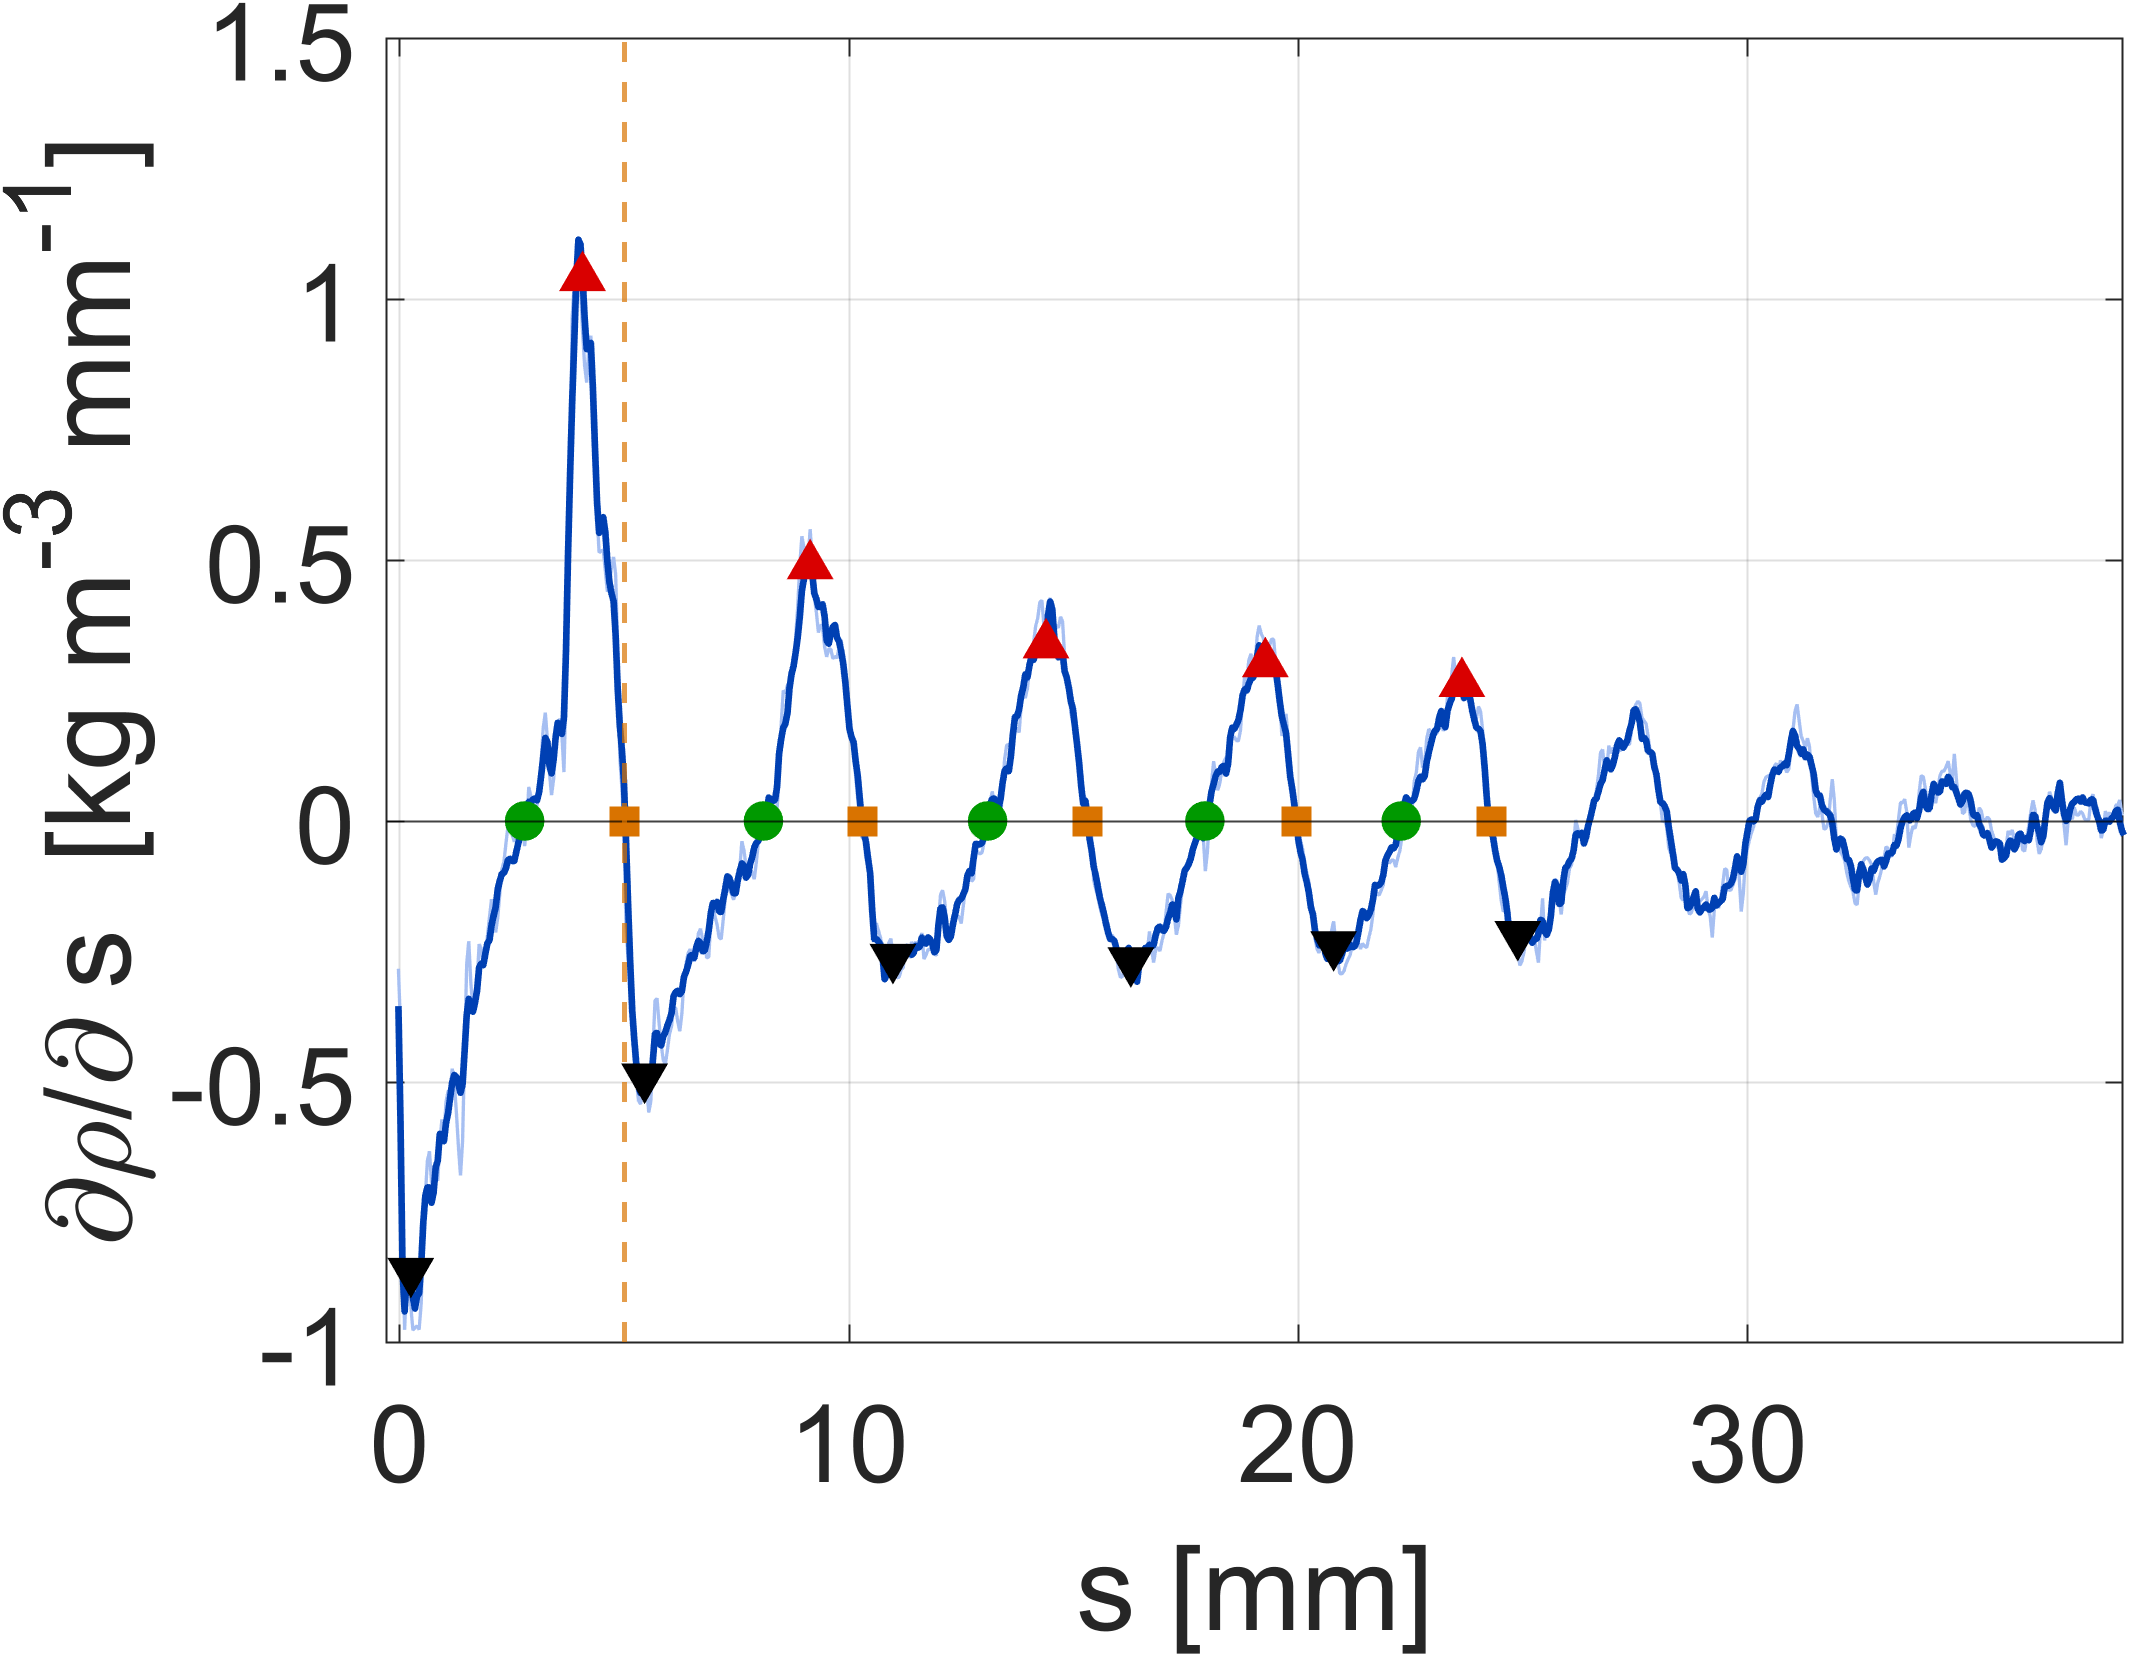
\includegraphics[width=\textwidth]{figures/centerline density gradient dataset f.png}
        \caption{Dataset f, with respective $NPR = 3.875$ and $L_s = 5.00$ mm}
        \label{fig: centerline density gradient dataset f}
    \end{subfigure}
    \caption{Centerline density gradient in the s direction for datasets a to f, obtained assuming a planar field. The light blue line is the gradient at the axis row $n = 0$ and the dark blue line its mean over $|n| \leq 0.25$ mm. Red upward triangles mark the compression peaks, black downward triangles the expansion valleys, green circles the density minima and orange squares the density maxima detected along the centerline. The dashed orange line marks the end of the first shock cell, $L_s$}
    \label{fig: centerline density gradients}
\end{figure}

% REVIEW: L_s is defined here as the distance between consecutive maxima, but the caption and the values use the nozzle to the first maximum. The NPR used for the fit comes from the shear layer angle, so the literature comparison checks consistency rather than validating the NPR independently.
The 6 plots in Figure \ref{fig: centerline density gradients} allow the identification of important marks in the shock cell structure. The periodicity and dissipation effect is clear, each cell is marked by an expansion valley and a compression peak and its amplitude decreases until atmospheric conditions are reached. The density maxima and minima are also distinguishable as the points where the gradient is zero. The distance between two consecutive maxima marks the length of the shock cell. For each dataset, the lengths of the first shock cell $L_s$ have been retrieved and they are displayed in their respective plot caption. The data confirms the previous qualitative visual evaluations regarding the shock cells sizes, as it shows that $L_s$ increases monotonically with $NPR$, meaning that the shock cells stretch further at increasing nozzle pressure ratios. It is also notable that more cells are present at higher pressures. Now that a more realistic estimate of the $NPR$ and $L_s$ have been achieved, it is possible to correlate both quantities using the formats of Equations \ref{equation: Emden Formula} and \ref{equation: Lazarus-Hartmann Formula} and compare to Emden's and Hartmann-Lazarus' formulation respectively, this way validating the application with literature data.

%Add shock cell length picture 

% REVIEW: Figure \ref{} is empty. The fitted L_s is the first cell, but Emden k = 0.88, Prandtl k = 1.2 and Hartmann-Lazarus k = 1.06 describe the later cells (average of later cells?); only the Hartmann-Lazarus constant-term formula (0.98, 0.30) is for the first cell. "Can be said to be satisfactory" is weak for a conclusion.
The fitted curves using Emden's and Hartmann-Lazarus' formulations are displayed together with the literature solutions in Figure \ref{}. The obtained values for the constants are: $k = 1.16, a = 0.894$ and $b = 0.28$. The $k$ value differs from Emden's $0.88$ figure, however, it is in line with other estimates such as Prandtl-Pack's $k = 1.2$ and Hartmann-Lazarus' $k= 1.06$ \cite{Emden1899, Hartmann1941, Powell2010}. Visually, the data is positioned in-between Hartmann-Lazarus' equation and Emden's formulation, as it slightly underestimates the former and considerably overestimates the latter. Regarding the fits, the Hartmann-Lazarus equation better describes the data behavior as the Emden format diverges significantly to the last point. Given that the data follows a trend format previously observed in the literature, is positioned in between two established results, and given the limitations of the measurements, the results can be said to be satisfactory.

\subsection{Quantitative Density Field results}
\label{subsection: Quantitative Density Field results}

One of the goals of the compressible jet experiment was the quantitative reproduction of its density field using the displacement data gathered with SBOS. In order to achieve that, the vector field had to go through a series of post-processing steps, integration schemes and noise regularization. The first ones were already mentioned, where the median of the background vector was removed and the image translated and rotated to position the jet axis horizontally at n = 0. Furthermore, the resulting displacements were averaged folded along n = 0. For the even function $\partial \rho / \partial s$  the symmetric components were summed and halved, while for the odd function $\partial \rho / \partial n$ the sum of the absolute symmetric components was halved. Placing the jet axis at n = 0 and folding it is of utmost importance for the implementation of the next step, as any anti-axissymetric feature will introduce errors. Next, an Abel inversion algorithm was implemented following the integration and inversion steps in the theory of section \ref{subsection: Axisymmetric Refractive Field}. An onion-peeling integration method described by Dasch \cite{} was implemented, together with a Tikhonov regularization scheme to smooth out noise, as studied by Daun \cite{}, with Generalized Cross Verification of Golub \cite{} to choose the Tikhonov parameter.

\section{Aerospike Experiment Results}